\documentclass[review]{elsarticle}

%\documentclass[1p,review]{elsarticle}
\usepackage{pifont}
\usepackage{booktabs}
\usepackage{natbib}
\usepackage{blkarray}
\usepackage{caption} 
\usepackage{multirow}
\usepackage{graphicx}
\usepackage{float}
\usepackage{amsmath}%
\usepackage{amsfonts}%
\usepackage{amssymb}%
\usepackage{graphicx}
\usepackage{pdflscape}
\usepackage{tablefootnote}
\usepackage{array}
\usepackage{framed}
\usepackage{setspace}
\usepackage[margin=3cm]{geometry} %changed from 2.5cm to 3cm so that margin notes don't get cut off.
\usepackage{graphicx}
\usepackage{caption}
\usepackage{subcaption}
\usepackage{natbib}
\usepackage{bibentry}
\usepackage{blkarray}
\usepackage{caption} 
\usepackage{multirow}
\usepackage{graphicx}
\usepackage{float}
\usepackage{amsmath}%
\usepackage{amsfonts}%
\usepackage{amssymb}%
\usepackage{tablefootnote}
\usepackage{array}
\usepackage{setspace}
\usepackage[mathlines]{lineno}
\usepackage{geometry}
\usepackage{url}
%\usepackage{subcaption}
%\usepackage{pdflscape}
\usepackage{lineno}
\usepackage{xargs}
\usepackage{amsthm}
\usepackage{graphics}
\usepackage[usenames,dvipsnames]{color}
\usepackage{enumerate}
\usepackage{dsfont}
\usepackage{tabularx}
\usepackage{tikz}\usetikzlibrary{shapes,arrows,positioning,calc,fit}



%%%%% BEGIN MIKE'S COMMANDS %%%%%
\usepackage[normalem]{ulem}  %provides strikeout \sout{}
\usepackage{xspace} %%needed for mike's commands

\newcommand\mymarginpar[1]{\marginpar{\begin{spacing}{0.7}\singlespacing \tiny #1 \end{spacing}}}  %for notes in margin

%%custom commands for sanity
\newcommand{\imax}{\ensuremath{i_{\max}}\xspace}
\newcommand{\mvec}{\ensuremath{\vec{m}}\xspace}
\newcommand{\mstarvec}{\ensuremath{\vec{m}}\xspace}
\newcommand{\GCD}{\ensuremath{\text{GCD}}\xspace}
\newcommand{\detA[1]}{\ensuremath{\ensuremath{\det\left[\bs{A}_{#1}\right]}\xspace}}

\doublespacing


%%%%% END MIKE'S COMMANDS %%%%%




%----------------------------------------------------------
\biboptions{round,authoryear}
\AtBeginDocument{\renewcommand{\bibname}{References}}
\renewcommand{\floatpagefraction}{0.1}
\newcolumntype{L}[1]{>{\raggedright\let\newline\\\arraybackslash\hspace{0pt}}m{#1}}
\newcolumntype{C}[1]{>{\centering\let\newline\\\arraybackslash\hspace{0pt}}m{#1}}
\newcolumntype{R}[1]{>{\raggedleft\let\newline\\\arraybackslash\hspace{0pt}}m{#1}}
\floatstyle{plaintop}
\restylefloat{table}
\restylefloat{figure}

%Quicklimit
\newcommand\limf[1]{\lim_{#1 \to \infty}}
%quick partials
\newcommand\p[2]{\frac{\partial #1}{\partial #2}}
\newcommand\ptwo[2]{\frac{\partial^2 #1}{\partial #2^2}}
\newcommand\mptwo[3]{\frac{\partial^2 #1}{\partial #2 \partial #3}}
%var text
\newcommand{\var}{\mathrm{var}}
%indicator
\newcommand\ind[1]{\mathds{1}_{\{#1\}}}
\newcommandx{\iton}[3][1=i,2=1,3=n]{_{#1 = #2}^{#3}}
%Norm Distrubtion
\newcommand\isnorm{\sim N(\gm,\gs^{2})}
\newcommand\issnorm{\sim N(0,1)}
\newcommand\isnormd[2]{\sim N(#1,#2)}
\newcommand\isbeta{\sim Beta(\alpha,\beta)}
\newcommand\isbetad[2]{\sim Beta(#1,#2)}
%----
\newcolumntype{A}{ >{$} r <{$} @{} >{${}} l <{$} } % A for "align"
%% (1) "r" column in math mode:          >{$} r <{$}
%% (2) no space:                         @{}
%% (3) "l" column in math mode, with 
%%     an empty subformula at the start: >{${}} l <{$}


%----


%\captionsetup[table]{skip=10pt}
%\setlength\belowcaptionskip{5pt}
\renewcommand{\arraystretch}{1.5}
\newtheorem{acknowledgement}{Acknowledgement}
\newtheorem{algorithm}{Algorithm}
\newtheorem{axiom}{Axiom}
\newtheorem{case}{Case}
\newtheorem{claim}{Claim}
\newtheorem{conclusion}{Conclusion}
\newtheorem{condition}{Condition}
\newtheorem{conjecture}{Conjecture}
\newtheorem{corollary}{Corollary}
\newtheorem{criterion}{Criterion}
\newtheorem{definition}{Definition}
\newtheorem{example}{Example}
\newtheorem{exercise}{Exercise}
\newtheorem{lemma}{Lemma}
\newtheorem{notation}{Notation}
\newtheorem{problem}{Problem}
\newtheorem{proposition}{Proposition}
\newtheorem{remark}{Remark}
\newtheorem{solution}{Solution}
\newtheorem{summary}{Summary}
\newtheorem{theorem}{Theorem}
\newtheorem{excont}{Example}
\renewcommand{\theexcont}{\theexample}
%\numberwithin{equation}{subsection}
%\numberwithin{example}{section}
\newcounter{exampleEq}
%-----------------------------------------------------------
\let\bs\boldsymbol
%----
%----
%----
\makeatletter
\@fpsep\textheight
\makeatother

%-- Flow Chart Definitions -----------------------------------------
\tikzstyle{cloud} = [rectangle, draw, fill=red!20, inner sep=0.25em, text width=5em, text centered, rounded corners, minimum height=4em, execute at begin node=\scriptsize]
\tikzstyle{subcloud} = [rectangle, draw, fill=green!20, inner sep=0.5em, text width=8em, text centered, rounded corners, minimum height=3em, execute at begin node=\scriptsize]
\tikzstyle{block} = [rectangle, draw, fill=blue!20, inner sep=0.5em, text width=13em, align=center, minimum height=3em, execute at begin node=\scriptsize]
\tikzstyle{light} = [rectangle, draw, fill=blue!10, inner sep=0.5em, text width=9em, text centered, minimum height=1em, execute at begin node=\tiny]
\tikzstyle{io} = [trapezium, draw, fill=green!20, trapezium left angle=70, trapezium right angle=-70, inner sep=0.5em, text width=5em, text centered, minimum height=3em, execute at begin node=\scriptsize]
\tikzstyle{decision} = [diamond, draw, fill=yellow!20, inner sep=0.05em, aspect=2, text width=4em, text badly centered, minimum height=5em, minimum width=7em, rounded corners, execute at begin node=\tiny]
\tikzstyle{query} = [rectangle, draw, fill=red!20, inner sep=0.5em, text width=5em, text centered, minimum height=3em, execute at begin node=\scriptsize]
\tikzstyle{prompt} = [trapezium, draw, fill=green!20, trapezium left angle=60, trapezium right angle=60, inner sep=0.5em, text width=5em, text centered, minimum height=3em, execute at begin node=\scriptsize]
\tikzstyle{stop} = [regular polygon, regular polygon sides=8, draw, fill=red!20, inner sep=0.05em, text width=5em, text centered, execute at begin node=\scriptsize]
\tikzstyle{go} = [circle, draw, fill=green!20, inner sep=0.5em, text width=5em, text centered, rounded corners, minimum height=3em, execute at begin node=\scriptsize]


\tikzstyle{line} = [draw, -latex']
\tikzstyle{noarrow} = [draw]
\tikzstyle{container} = [rectangle, draw, inner sep=0.4em, dashed, fill=none, color=red!40]



\begin{document}
\title{Modeling mRNA Populations}
\author[utkm,curradd]{N.~Pollesch\corref{cor1}}
\ead{pollesch@math.utk.edu}
\author[utkgst]{Ricardo Urquidi}
\author[utkeeb,nimbios,cor1]{M.A.~Gilchrist}
\ead{mikeg@utk.edu}
\cortext[cor1]{Corresponding author}
\address[utkm]{Department of Mathematics, University of Tennessee,  Knoxville, TN 37996-1320}
\address[utkeeb]{Department of Ecology and Evolutionary Biology, University of Tennessee, Knoxville, TN 37996-1610}
\address[nimbios]{National Institute for Mathematical and Biological Synthesis, University of Tennessee, Knoxville, TN 37996-3410}
\address[utkgst]{Genome Science and Technology Program, University of Tennessee, Knoxville, TN 37996-XXX}

\begin{abstract}
This paper presents a model to describe the dynamics of protein translation.  
A system of ordinary differential equations is derived to describe the number of ribosomes bound to a strand of mRNA at a given time.
The number of ribosomes bound to an mRNA at a given time is referred to its ribosome load.
The mRNA is classified based on its ribosome load and whether or not it's decapped for future degradation.  
Distribution of ribosome counts is assumed to be related to the translation initiation rate, translation completion rate, degredation marking rate, and length of the mRNA.
%The proposed marking phenomena leads to natural division of the state variables in capped and decapped classes.
The length of the mRNA's coding region plays the role of controlling the number of ribosome counts which, in turn, determines the number of ODEs in the system.  
%This maximum number of ribosomes that can be bound at any given time as a function of gene length is denoted as \imax.
A goal of this work is to see how the equilibrium distribution between classes as changes with coding region length.
A closed form solution to the density in the $i^{th}$ ribosomal class in a system with \imax states is presented for the equilibrium distribution of the decapped classes in terms of the capped classes.
The equilibrium solutions in the capped classes are shown to be related to the full determinant of the tri-diagonal matrix used to describe the system, as well as all the determinants of the minors associated to it.
In general, there is no closed form for the determinant of a tri-diagonal matrix, only a recurrence relation that can be used to find determinants.
However, in this model a closed form exists for the full determinant as it changes with changing values of \imax and its formula is presented .
This closed form for the determinant provides a method to efficiently find equilibrium solutions for the entire system.
Additionally, a continuous approximation using PDE is derived and also used to find equilibrium solutions to the system.
Both of these methods for determining equilibrium solutions are utilized in an effort to find the set of parameters that maximizes the likelihood of a given data set.
A process for mapping the equilibrium model results to data is also presented and used to begin preliminary estimation of model parameters and to verify model function.
 
\textbf{alternate abstract: Modeling Ribosomal Loading of mRNA}\\
A model is presented to describe the dynamics of protein translation related to the ribosomal load of an mRNA.
The number of ribosomes bound at a given time is referred to as ribosome load, and using this value a population of mRNA are classified.
A system of ordinary differential equations (ODEs) is derived and solved for the equilibrium distribution of a population of mRNA.
Distribution of ribosome counts is assumed to be related to the translation initiation rate, translation completion rate, degradation marking rate, and length of the mRNA.
Methods are developed to find analytical equilibrium solutions to the system of ODEs and a system of partial differential equations (PDEs) are derived to find numerical approximations to the ODE system at equilibrium as well.
Both the PDE continuous approximation and the analytical solutions to the ODE system agree offering two different methods for finding solutions at equilibrium within optimization routines.
Additionally, a tool is developed and presented that is used to compare the model results to empirical microarray data measures of ribosome load.  
\end{abstract}
\begin{keyword}
bioinformatics \sep mRNA population \sep protein translation \sep ribosome loading \sep ribosome count \sep polysome \sep mathematical model
\end{keyword}
\maketitle
%\newpage
%\tableofcontents
\newpage

\textbf{Paper Outline}
\begin{enumerate}
\item Motivation - \textbf{(Mike)}
\begin{enumerate}
\item Why is this process important?
\item What will this model enable researchers to do?
\item Other modeling efforts?
\end{enumerate}
\item Derivation and Assumptions
\begin{enumerate}
\item Physical processes captured (Ideally, have a quick discussion of process and inline definitions of variables used to represent process, followed by a total recap in a table)  - \textbf{(Nate)}
\begin{enumerate}
\item System described as population model: Dichotomy of decapped and capped mRNA.
State variables based on an mRNA's ribosome load.
\item Process of mRNA production
\item Process of Marking mRNA for degradation supposed
\item Three processes of : Initiation, translation, and completion
%\item Originally included total number of ribosomes in system, but has since been excluded.
\end{enumerate}
\item Definition/Discussion of system boundaries - (\textbf{MIKE})
\begin{enumerate}
\item Physical boundaries as a cell and relation to parameters
\item Discussion of perceived upper and lower limits to state variables and parameters
\item Temporal boundaries and relation to steady state
\end{enumerate}
\item Assumptions: Such as initial assumptions of specific functional forms, i.e. marking rate constant among classes  - \textbf{(Nate)}
\item Justify consideration of system as two subsystems, decapped and capped.  - \textbf{(Nate)}
\end{enumerate}
\item Model Formulation: Total model presented and then analysis of capped and decapped systems  - \textbf{(Nate)}
\begin{enumerate}
\item ODE/Discrete system
\begin{enumerate}
\item Present system of ODEs (Total, capped, and decapped)
\item Matrix Representation of ODE model (Total, capped, and decapped)
\item Steady state formulations
%\item (Make decision to present results for steady state values for ODE here or after formulation of PDE system in a results section)
\end{enumerate}
\item PDE/Continuous system 
\begin{enumerate}
\item Explain motivation for deriving PDE
\item Explain framing as `non-linear birth and death process'
\item Explain derivation using Taylor expansion
\item Present PDE for capped class
\item Present non-dimensionalized system
\item Present 2nd order ODE to be solved for non-dimensionalized PDE at Equilibrium
\item Motivate and present equation for decapped class at equilibrium
\item (Make decision to present results for steady state values for PDE here or in a separate section to follow)
\end{enumerate}
\end{enumerate}
\item Results  - \textbf{(Nate)}
\begin{enumerate}
\item Present solution strategies/methods
\begin{enumerate}
\item ODE/Discrete system: Matrix inversion technique
\item PDE/Continuous system: Numerical solver of 2nd order ODE that arises at equilibrium
\item Discussion of alternative solution approaches
\end{enumerate}
\item Present actual solutions for a couple sets of parameters: Highlight agreement of ODE and PDE system
\item Present solutions for discrete system under further simplifications for translation and initiation
\end{enumerate}
\item Opportunities for Future Research  - \textbf{(Nate and Mike)}
\begin{enumerate}
\item Application of model to real data.
Can highlight sources of data.
\item Alternate functional forms and relaxed assumptions
\item Further establish connection (in simplified system) to potential probability distributions
\item How to move forward with analytical solutions, specifically connection to solving 2nd order partial difference equation arising from tri-diagonal form of matrix, note here that boundary conditions exist that may be utilized which are not normally present.
\end{enumerate}
\end{enumerate}
\newpage
\section{Introduction}
This section addresses such topics as why modeling this process important, what this model will enable researchers to do, and what other modeling efforts exist that seek to achieve the same goals.

\subsection{mRNA and Translation}\label{sec:Bioligical underpinnings}
%description of the biological underpinnings of the model.
%T


\begin{enumerate}%rough ideas / poteintially important concepts
	\item Gene expression short overview
	\begin{enumerate}
		\item Gene expression is often stated as the central dogma in which genetic information encoded in the DNA is transcribed into mRNA which is subsequently translated into protein. 
		\item Often, a greater amount of attention is focused on explaining gene expression at the transcriptional level and prevailing changes of mRNA transcript levels. 
		\item However, multiple studies across all kingdoms of life have shown that transcript expression level is only moderately predictive of the final protein expression.
		\item Gene expression at the post transcriptional level is controlled by mRNA transcript stability and degradation, translation and protein maturation/degradation.
		\item The model presented in this paper encompasses gene expression regulation occuring at the translational and the mature mRNA population level.
	\end{enumerate}
	\item Biology controlling mRNA stability and translation
	\begin{enumerate}
		\item Mature mRNAs in the cytosol are called the free mRNA pool, and are in one of three states. 
		\item They are actively being translated by ribosomes and will continue to initiate new rounds of translation until the transcript is degraded.
		\item Transcripts are degraded directly from the free mRNA pool.
		\item Transcripts are protected from degradation by RNA binding protein chaperones or are found in processesing bodies awaiting translation initiation or degradation.
		\item Degradation of mature mRNAs is controlled by numerous processes depending on whether they are bound to ribosome, in processing bodies or in the free mRNA pool.
		\item Free mRNAs can be decapped or deadenylated followed by exonuclease digestion.
		\item Ribosomes can destine transcripts to degradation under multiple conditions. 
		\item The first ribosome to bind to a freshly exported transcript performs the "pioneer round of translation", which is charged with assesing the mRNA's quality.
		\item There are 3 processes which occur in the pioneer round of translation, all of which detect different mRNA defects. 
		\item No Go Decay (NGD) detects a stalled ribosome, either due to mRNA structural features, slowly translating sequence or inteference of translation elongation. %sRNA interference has been suggested, need to read sources
		\item No stop decay (NSD) detects a missing stop codon and nonsense mediated decay (NMD)  detects potential mis splicing or nonsense mutations.
		\item All three decay  mechanisms, NMD, NSD and NGD lead to the eventual degradation of their bound transcripts. 
		\item While NSD and NMD are a restricted to the pioneering round of translation, NGD can also uccur during the following rounds of translation.
		\item As transcripts are cleared by the pioneering round of translations more ribosomes can attach to the transcript, once more than one ribosome is on a transcript this ribosome mRNA complex is called a polysome.
		\item Transcripts associated to ribosomes are generally assumed to be protected from degradation and only degraded once ribosomes are off the transcript, however both NGD, (sRNA silencing) and 
			a process called cotranslational decay can degrade actively translated transcripts.
		\item Cotranslational decay involved the decapping of actively translating mRNA transcripts and subsequent 5' to 3' mRNA degradation which follows a 3 nucleotide periodic pattern in step with the Ribosome.   
	\end{enumerate}
	\item Current Models/Research and how our model fits in the current field

\end{enumerate}

\begin{enumerate}
% This is material for the intro. but I need it to properly contextualize the introduction of the model and figure 1%
	\item  The basic representation of the central dogma dictates that epression of protein coding genes starts from genes encoded in DNA that are transcribed to mRNA and subsequently translated to Protein.
 	\item A more careful representation considers that the final protein production is dependent on both the maintenance of an actively translating mRNA population, the association of ribosomes on the population and finally the degradation of the protein itself.
	\item The maintenance of mRNA populations relies on the balance of mRNA transcription rates, the translation status of transcripts and numerous mRNA decay pathways.
	\item mRNA degradation relies on removing protective and translation enhancing componenets of the mRNA. These include the 5' mG cap and the 3' polyadenosine tail.   
	\item Additionally mRNA degradation can be promoted through endonucleolytic cleavage by RISC (and siRNAs).
	\item mRNA degradation can occur in both a ribosomal associated or a ribosome free manner.
	\item Ribosomal association of transcripts can lead to both protection of viable transcripts as well as quality control degradation of faulty transcripts. 
	\item When a viable transcript is bound by the ribosomal and translational machinery, the 5' cap is bound by translational initation factors and the 3' tail is bound by poly A binding proteins. This protects transcripts from exonucleic attack and degradation.
	\item Endonucleic degradation is still possible, but reduced due to a reduced accessibility of the siRNA binding sequence on the transcript through competition with ribosomes.
	\item However multiple mechanisms of mRNA decay are carried out in association with the ribosome. Nonsense mediated decay, no go decay and no stop decay all rely on ribosomes detecting faults in the transcript and susbsequently interacting with degradation machinery to remove the faulty transcript.
	\item With some mechanisms of mRNA decay, decay can occur co-translationally. This is mainly seen in 5' decapping. When a translating transcript is decapped the 5' to 3' exonucleic degradation machinery trails the most upstream ribosome. As the ribosome translates the mRNA is degraded.
	\item 

\end{enumerate}




\section{Methods}\label{sec:description}
%A model of mRNA populations under control of translation and co-translational decay
\subsection{Model Overview}
\pagebreak
\begin{figure}[!ht]
\centering
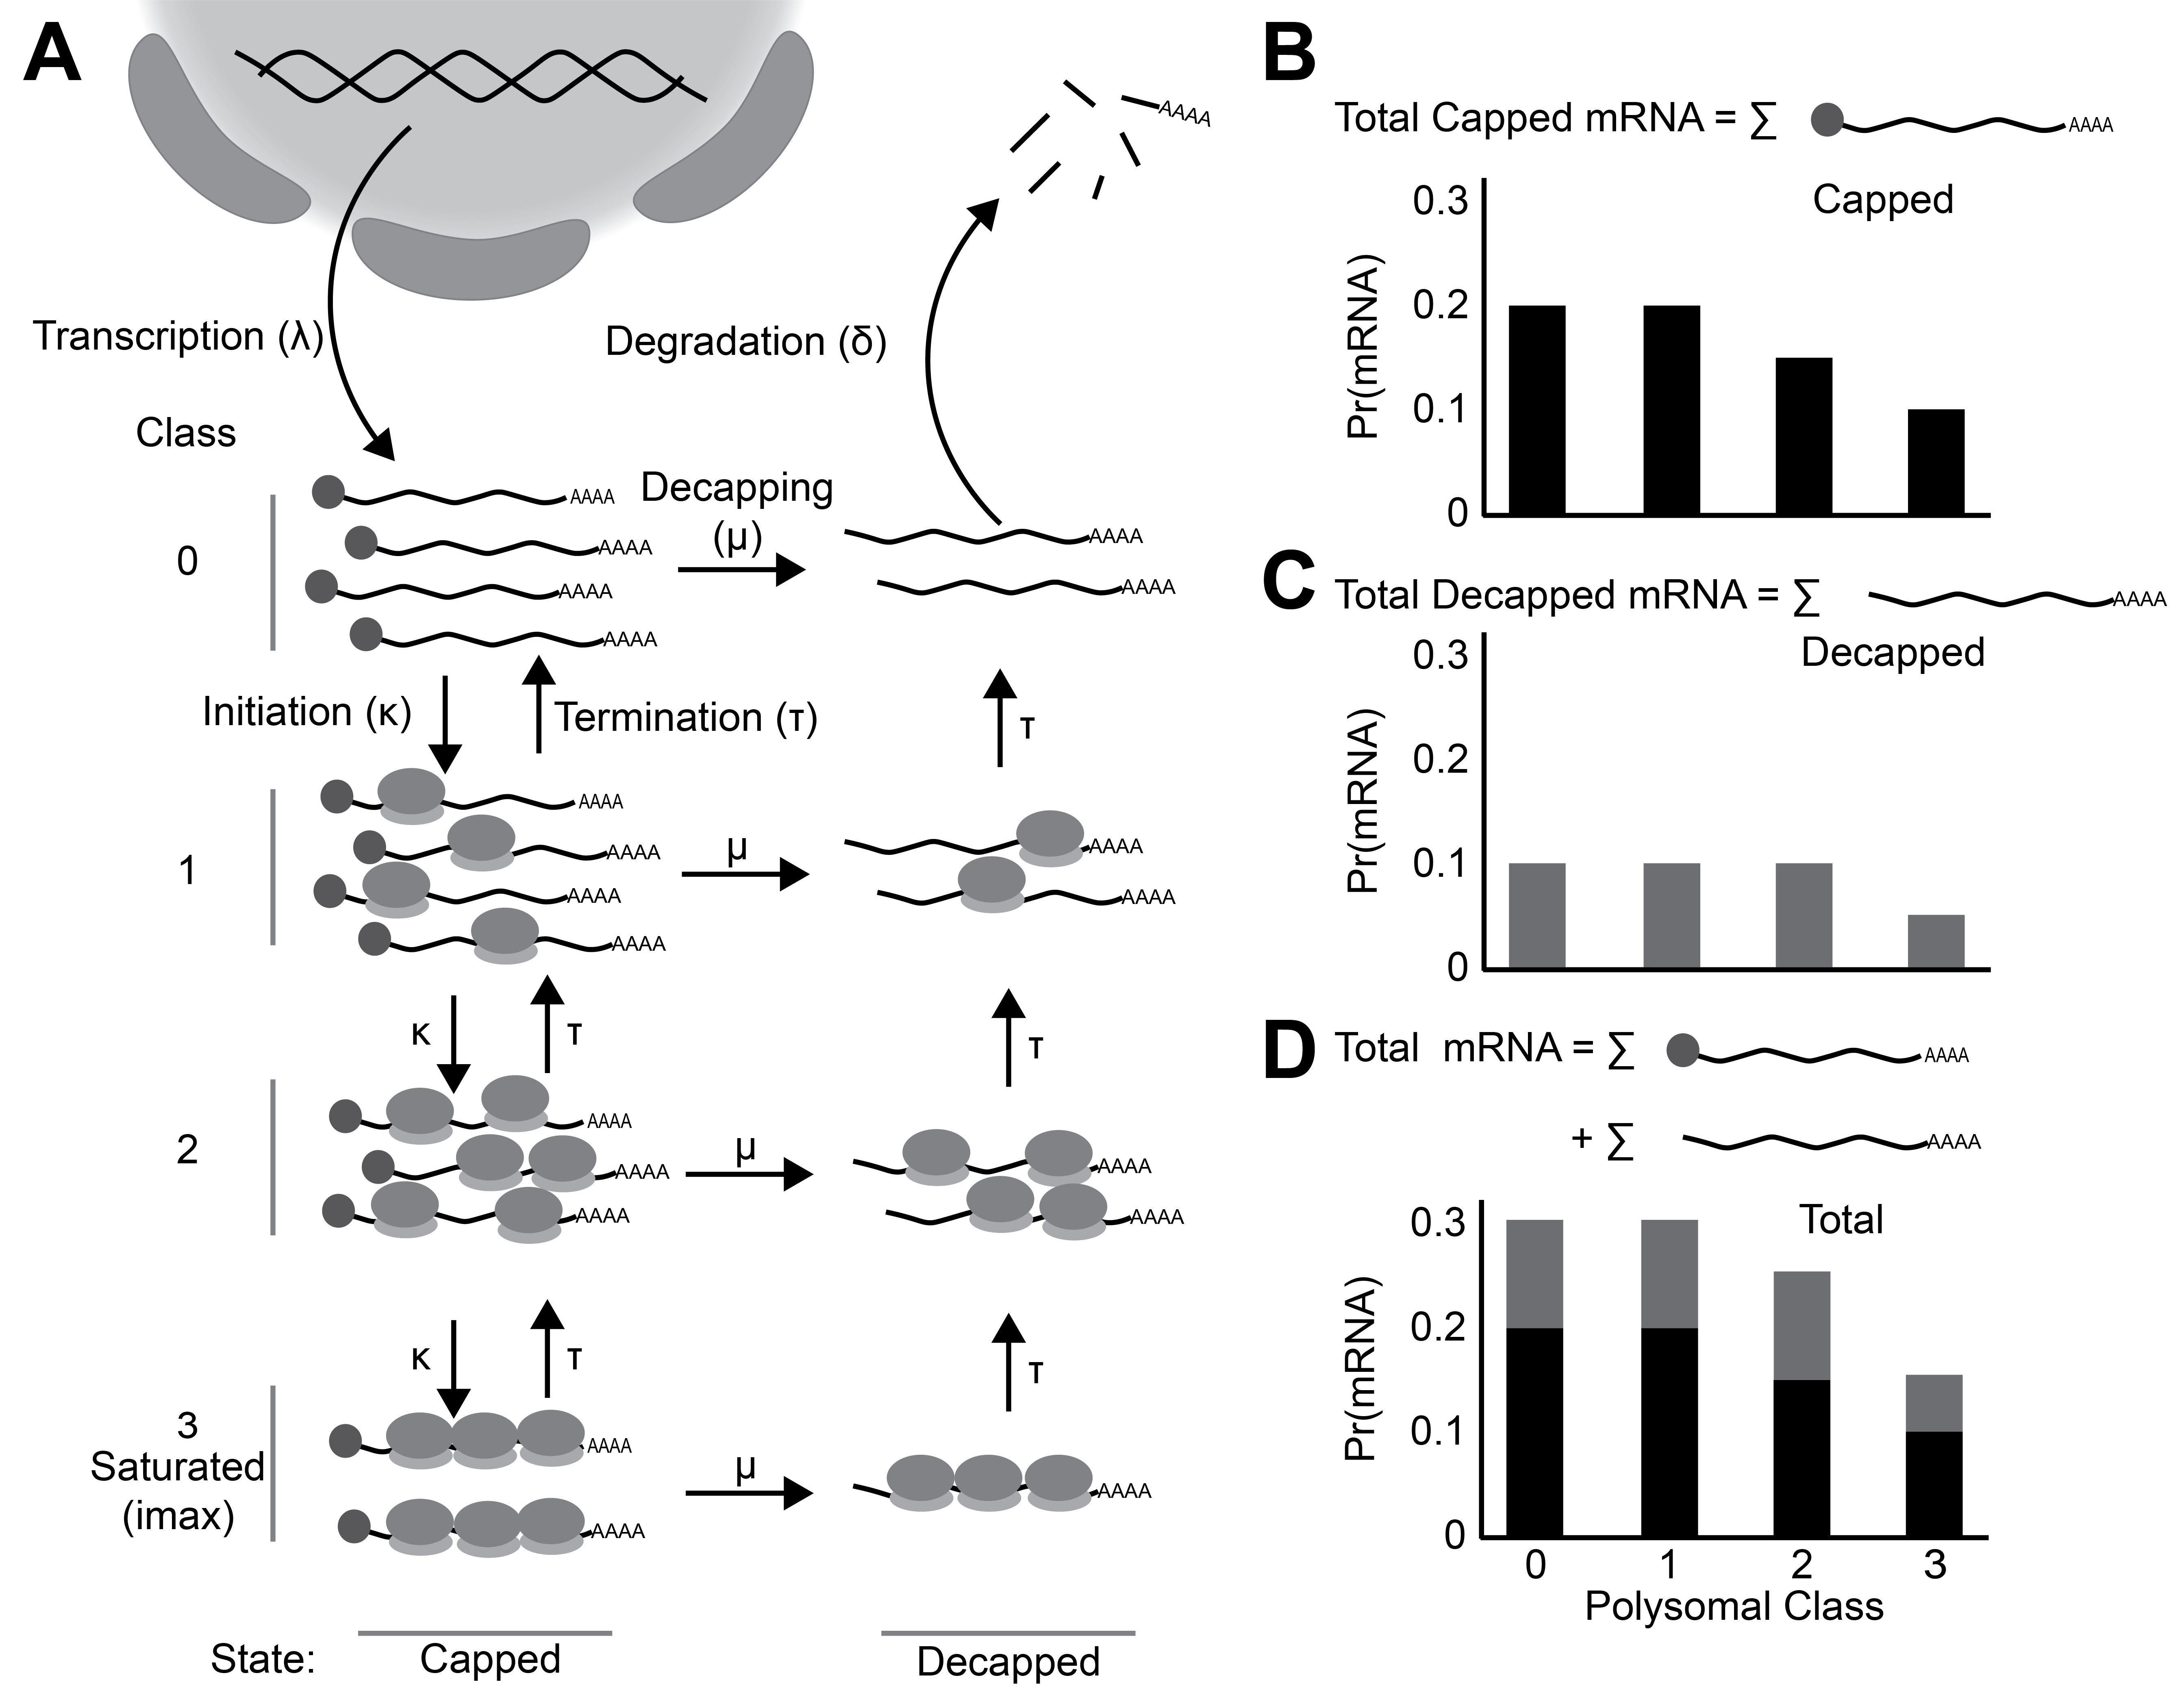
\includegraphics[width=150mm]{Images/Figure1_biomodel_V3.png}
\caption{Cartoon Representation of model in biological context. A) Model overview. Transcripts enter the sytem into the capped state at class 0 (no ribosomes bound). They enter the state at rate $\lambda$ through transcription. Transcripts are free to move up and down ribosomal classes at rates $\kappa$ for translation initiation and $\tau$ for elongation/termination. Transcripts can also be decapped and enter the decapped state at rate $\mu$. Finally, upon reaching class 0 in the decapped state transcripts are fully degraded at rate $\delta$. B) Probability of finding an mRNA in each class in the capped state. C) probability of finding an mRNA in each class in the decapped state. D) Joint probabilty of finding an mRNA in each class across each state. This reflect the total protein production potential.}
\end{figure}
\pagebreak


The model captures some of the basic processes governing mRNA populations: transcript production, degradation and the process of translation (Figure 1A).
Transcripts can exist in one of two states: capped and decapped which captures the the role of the 5' cap in mRNA protection and translation initiation. 
Capped transcripts are translationally competent, meaning that new ribosome can be loaded onto the transcript. 
Individual transcripts in the cell will be found with a set number of ribosomes (none, 1, 2, etc).
The number of ribosomes on a transcript determines that transcripts ribosomal class.
The model seeks to determine how the population of transcipts of a single gene are distributed between ribosomal classes and capped and decapped states.
Transcripts enter into the model as defined by the transcription rate $\lambda$ into the capped state with no ribosomes (class 0)
From capped class 0 a transcript can have two fates. 
The transcript can be decapped for degradation at rate $\mu$ and move into the decapped class 0.
Alternatively, a ribosome can initiate translation at rate $\kappa*(1-i/imax)$ and be loaded onto the transcript and move it into capped class 1.Where i is the current transcript class and imax is the maximal ribosomal occupancy on the transcript
A ribosome on transcript can then elongate and terminate at a rate of $\tau * i$. After a ribosome fully elongates and terminates it leaves the transcript and the transcript falls to a lower class.
Capped transcripts move through rounds of translation initiation and elongation\/termination and distribute along the different ribosomal classes. 
From any ribosomal class in the capped state the transcript can be decapped at rate $\mu$  and move into the decapped state while maintaining the same ribosomal class.
decapped transcripts can no longer initate new rounds of translation, but allow for currently loaded ribosomes to complete translation. 
This process represent co-translational decay, a common method of mRNA decay in eukaryots (Citation) 
After all ribosome complete translation, the mRNA is in decapped class 0 and completely degraded at a rate $\delta$.
The saturated state of a transcript is denoted as \emph{imax}, meaning that that transcript can no longer accept any more ribosomes. 
The model produces two outputs. 
First, the total mRNA in each state and therefore the system (Figure 1B-D). 
Second, The distribution of the mRNAs in each mRNA in each ribosomal class. (Figure 1 B-D).
The total protein output at steady state from our model can be obtrained by calculating the average ribosomal class in the system by the total mRNA in the system (Figure 1D). 

\subsection{Model Definition and Analysis}
For simplicity, we begin by defining our model equations using generic functions to describe the transition of mRNAs between different classes or states.
We then constrain the model by assuming specific functions to describe the transition of mRNAs between classes.
%Note that from here forward the capped and decapped subsystems are presented separately, the benefits of taking this approach will become evident as we proceed.  

\subsection*{General model equations of the density independent initation model}
%\subsection{The capped subsystem}
Our model consists of two sets of time dependent and coupled ODEs.
Each set of ODEs describes the abundance of mRNAs that are either capped and decapped for degradation.
The ODEs within each sets equations are structured by the ribosome load of the mRNA.
The coupled ODEs within a set of equations describe how mRNAs are introduced to the set, the transitions in ribosome load via initiation or completion of protein translation,  and the transition between sets either via the marking of capped mRNAs or the degradation of decapped mRNAs with a ribosome load of 0.

\begin{table}
\centering
\begin{tabular}{|rp{4in}|c|c|c|}\hline
\textbf{Symbol}&\textbf{Description}&\textbf{Unit} \\\hline
State Variables & &  \\ \hline
$m_i$ & Abundance of mRNAs with a ribosome load of $i$ in capped state. & $mRNA$ \\
$m_i^*$ & Abundance of mRNAs with a ribosome load of $i$ in decapped state. & $mRNA$ \\ \hline
\multicolumn{1}{l}{Model Parameters} \\ \hline
  \imax & \shortstack{Maximum number of ribosomes able to bind to mRNA;\\
           defines number of state variables and is a function of gene length.} & ND \\
$\kappa(i)$ & Translation initiation rate for unmarked mRNAs with a ribosome load of $i$. & $1/s$\\
$\tau(i)$ & Translation completion rate for the marked and unmarked mRNAs with a ribosome load of $i$. & $1/s$\\
$\mu(i)$ & Marking rate for unmarked mRNAs with a ribosome load of $i$. & $1/s$\\
$\lambda$ & Production rate of newly produced, ribosome free, and unmarked mRNA to the $m_0$ class. & $mRNA/s$\\
$\delta$ & Removal rate of marked mRNA with a ribosome load of 0 from the $m_0^*$ class. & $1/s$\\ \hline 
%\multicolumn{3}{|p{450pt}|}{\footnotesize Note: $\mathbb{R}^+$ represents the non-negative real numbers and $\mathbb{Z}^{(+)}$ represents the strictly positive integers.} \\ \hline
\end{tabular}
\caption{State variables and model parameters for ODE model of mRNA populations.
Variable \imax is in the domain of non-negative integers; all other variables are non-negative real numbers.}
\label{tab:params}
\end{table}

Specifically, new mRNA enter the $0^{th}$ capped class $m_0(t)$ at a rate..
Ribosomal bind mRNAs in the $i^{th}$ capped class at a rate $\kappa(i)$, increasing the mRNA's ribsome load to the $i+1^{th}$ class.
By definition, $\kappa(\imax)= 0$, i.e.~mRNAs with a ribosome load of \imax cannot accommodate any addtional mRNAs.
In the density independent model (DII), we assume that the current ribosomal load has no effect on the ability of another ribosome to bind to the transcript. 
An average ribosomal footprint covers 9 codons (~27 nucleotides). Therefore for a protein of 270 amino acids in length, the maximal ribsomal load, \imax = 10.
Capped mRNAs with ribosome load $i$ are decapped at a rate of $\mu(i)$.
We assume that capped mRNAs are decapped for degradation rate independent of their ribosome load, i.e. $\mu(i)=\mu_0$.
Accordingly, the ribosome load of decapped mRNAs remains unchanged, but they are transitioned from the capped class $m_i(t)$ to the decapped class $m_i^*(t)$ .
Ribosome movement along an mRNA is assumed to occur independent of whether or not its capped or decapped for degradation.
Thus, ribosomes complete translation of both decapped and capped mRNAs with ribosome load $i$ at rate $\tau(i)$, decreasing the mmRNA's ribosome load to the $i-1^{th}$ class. %class or state? State variables
Where $\tau(i)= i \cdot \tau(1)$ and .
This is because we not modeling the explicit movement of ribosomes along an mRNA, we assume that at steady state probability of finding a ribosome at any given codon position within the coding sequence follows a uniform distribution.
Thus, the chance that a ribosome on a transcript of class $i$ will complete translation increases as ribosome load increases.  
Since mRNA's with a ribosome load of 0 have no ribosomes which can complete translation, by definition $\tau(0) = 0$.
It is important to note that $\tau(1)$ is not the same as the average elongation rate. $\tau(1) = average \: elongation \: rate/(9 \cdot \imax)$. 
That is, the average elongation rate in $aa/s$ is rescaled to the average rate of total elongation and termination through a transcript in units of $1/s$.
At equilibrium every $\tau(i)$ must equal every $\kappa(i)$ by definition.  
Only mRNAs decapped for degradation and with a ribosome load of 0 are removed from the system.
Specifically, decapped mRNAs are removed from the $0^{th}$ class at a rate of $\delta \, m^*_0(t)$.
All parameters are assumed to fixed for a given gene, but may vary between genes.


The functional form of the capped subsystem is:
\begin{align*}
\frac{dm_{0}}{dt} &= \lambda+\tau(1)m_{1}-\left(\kappa(0) + \mu(0)\right)m_{0} \\
\frac{dm_{1}}{dt} &= \kappa(0)m_{0}+\tau(2)m_{2}-\left(\tau(1)+\kappa(1)+\mu(1)\right) m_{1}\\
& \vdots & \\
\frac{dm_{i}}{dt} &= \kappa(i-1)m_{i-1}+\tau(i+1)m_{i+1}-\left(\tau(i)+\kappa(i)+\mu(i)\right) m_{i} \\
& \vdots & \\
\frac{dm_{\imax}}{dt} &= \kappa(\imax-1)m_{\imax-1}-\left(\tau(\imax)+\mu(\imax)\right) m_{\imax}\\
\end{align*}

Similarly, the functional form of the decapped subsystem is:
\begin{align*}
\frac{dm_{0}^{*}}{dt} &= \mu(0)m_{0}+\tau(1)m_{1}^{*}-\delta m_{0}^{*} \\
\frac{dm_{1}^{*}}{dt} &= \mu(1)m_{1}+\tau(2)m_{2}^{*}-\tau(1)m_{1}^{*} \\
& \vdots & \\
\frac{dm_{i}^{*}}{dt} &= \mu(i)m_{i}+\tau(i+1)m_{i+1}^{*}-\tau(i)m_{i}^{*} \\
& \vdots & \\
\frac{dm_{\imax}^{*}}{dt} &= \mu(\imax)m_{\imax}^{*}-\tau(\imax)m_{\imax} \\
\end{align*}

\subsection{The density dependent initiation model}\label{sec:assumed_forms}
The DII model above is insensitive to the current ribosomal load on a transcript. 
But this doesn't mimic what happens in reality. Steric hindrance of recently initiated ribosomes prevent subsequent initiation.
This might be one explanation for the sometimes observed "translational ramp", a short strecth of amino acids right after the start codon which translate slower than the remaining transcript (Verma 2019). 
Specifically, we assume the start codon must be unoccupied by a ribosome in order for translation initiation to be successful.
As a consequence of this assumption, the probability of a ribosome occupying a given position on an mRNA with a ribosome load of $i$ is simply $i/\imax$.
Thus, the probability the start codon is unoccupied is $1-i/\imax$ and, in turn, our translation initiation rate function can be defined as, 
\begin{equation}\label{eq:kappa}
\kappa(i)=\kappa_0\left(1-\frac{i}{\imax}\right),
\end{equation} 
where $\kappa_0$ is a gene specific parameter that describes the rate at which capped mRNAs encounter and are bound by ribosomes within the cytosol (i.e.~it is an implicit function of the abundance of free ribosomes which we assume is constant).


%\mymarginpar{mikeg: 10/15/19: updated $\tau$ to explicitly include $1/imax$. Earlier notes indicate this term was implicitly absorbed into $\tau_0$.
 % mikeg: 10/22/19: updated to introduce $\tau^\prime_0$ and then reabsorb \imax into $\tau_0$ carrying this term through.
  %TODO update all later instances of $\tau_0$ with $\tau^\prime_0/\imax$ and then simplify math by canceling out \imax term and changing notation to remove the $\prime$ since it becomes unnecessary at that point.
  %mikeg: 03/11/21 Completed above changes (but haven't dealt with canceling)}
% \mymarginpar{Should this be $i/(\tau \imax)$?
%  On re-consideration that seems to sense since the probability a ribosome is at the final position is $1/\imax$.
%  However, I seem to recall deriving this result that indicate otherwise.
%  This shouldn't affect anything in this paper, but might explain some issues when fitting the data to model.
%  TODO for mike: Check notes.}
	%% Mike, the arguement for the derivation was as follows (if I remember correctly): For an mRNA with i ribosomes bound, it was assumed that each ribsome had an equal probability of being in any position, therefore, a ribosome was equally likely to be completing translation, therefore the probability of translation being completed was equal to the number of ribosomes bound, and thus the rate proportional to the number of ribosomes bound, leading to the form provided in eq:tau.  Does that stack up with what you were thinking?


Incorporating Equation 1 into the DII system yeild the density dependent intiation (DDI) model: %\subsubsection{The capped subsystem with Assumed Forms for $\kappa(i)$, $\tau(i)$, and $\mu(i)$}\label{sec:capped_simp}
\begin{align*}
\frac{dm_{0}}{dt} &= \lambda+\tau(1)m_{1}-\left(\kappa_0\left(1-\frac{0}{\imax}\right) + \mu(0)\right)m_{0} \\
\frac{dm_{1}}{dt} &= \kappa(0)m_{0}+\tau(2)m_{2}-\left(\tau(1)+\kappa_0\left(1-\frac{1}{\imax}\right)+\mu(1)\right) m_{1}\\
& \vdots & \\
\frac{dm_{i}}{dt} &= \kappa(i-1)m_{i-1}+\tau(i+1)m_{i+1}-\left(\tau(i)+\kappa_0\left(1-\frac{i-1}{\imax}\right)+\mu(i)\right) m_{i} \\
& \vdots & \\
\frac{dm_{\imax}}{dt} &= \kappa_0\left(1-\frac{\imax-1}{\imax}\right)m_{\imax-1}-\left(\tau(\imax)+\mu(\imax)\right) m_{\imax}\\
\end{align*}
and the decapped subsystem is unchanged.
%These equations are redundant. %%% NOT ADDRESSED AS OF 8/7 
\subsection{Matrix-vector Formulation of ODE System}
It is frequently useful to work with the matrix-vector formulation for a system of ODE.
In this model, the dynamics of the decapped and capped mRNAs can be represented as,
\begin{equation}\label{eq:matrix_full}\vec{M}'=\boldsymbol{F}\vec{M}+\vec{B},
\end{equation} 
where $\vec{M}\in\mathbb{R}^{2(\imax+1)}$ is a vector of all state variables, ordered here as $m_0$, $m_1$, ..., $m_{\imax}$, $m^*_0$, $m^*_1$, ..., $m^*_{\imax}$, $\vec{M}'$ is the vector containing the first derivatives of $\vec{M}$ with respect to time, $\bs{F}\in\mathbb{R}^{2(\imax+1)\times 2(\imax+1)}$ is the matrix representing the full system (Equation~\ref{eq:full_matrix}), and $\vec{B}\in\mathbb{R}^{2(\imax+1)}$ is the vector of $\lambda$ as the first component and 0s else.
Using the functional forms presented above, matrix formulations are provided next.

As opposed to explicitly listing elements of the full system matrix-vector representation we found that it is more convenient to utilize the block structure that emerges in this system and explicitly provide the block components.
The matrix $\bs{F}$ is block lower-diagonal and is given in Equation~\ref{eq:full_matrix}.
\begin{equation}
\label{eq:full_matrix}
\bs{F}=\left(\begin{array}{cc}
\bs{U} & \bs{0} \\
\bs{\mu} & \bs{R} \\
\end{array} \right).
\end{equation}
The upper-left block, $\bs{U}$, corresponds to the capped state variables, where $\bs{U}$'s general form is provided in Equation~\ref{eq:capped_matrix}.
The upper-right block is a matrix of all zeros, $\bs{0}\in\mathbb{R}^{\imax+1\times \imax+1}$.
Using $\bs{I}$ to represent the $\imax+1\times \imax+1$ identity matrix, the lower-left block is $\bs{\mu}=\mu_0\bs{I}$, a diagonal matrix with the constant $\mu_0$ on the diagonal and 0s else.
The lower-right block, $\bs{R}$, corresponds to the decapped state variables and its form is provided in Equation~\ref{eq:decapped_matrix}.

The matrix $\bs{U}$ is $(\imax+1\times \imax+1)$ dimensional and is tri-diagonal with non-zero entries on the diagonal, super-, and sub-diagonals,
\begin{equation}\label{eq:capped_matrix}
\bs{U}=\left(\begin{array}{cccccc}
-(\kappa_0+\mu_0) & \tau_0\frac{1}{\imax} &  &  &  & \\
\kappa_0 & \left(1-\frac{1}{\imax} \kappa_0+\mu_0+\tau_0\frac{1}{\imax}\right) & \tau_0\frac{2}{\imax} &  &  & \\
   &\ddots        & \ddots        & \ddots & &  \\
   & &    1-\frac{(i-1)}{\imax}\kappa_0 & -\left(1-\frac{i}{\imax}\kappa_0+\mu_0+\tau_0\frac{i}{\imax}\right) & \tau_0\frac{i+1}{\imax} & \\
                  &         &        & \ddots  & \ddots & \ddots \\
     
                          &        &  &  & \frac{1}{\imax}\kappa_0 & -\left(\mu_0+\tau_0\frac{\imax}{\imax}\right) \\
\end{array}\right).
\end{equation}
In the representation given in Equation~\ref{eq:capped_matrix}, all blank entries are 0.
The $(\imax-1)^{\text{th}}$ row has been suppressed in Equation~\ref{eq:capped_matrix}, but it can be generated using the formula included for the $i^{th}$ row.

The matrix $\bs{R}$ is the lower-right block in the block lower-diagonal matrix $\bs{F}$ (Equation~\ref{eq:full_matrix}),
\begin{equation}
\label{eq:decapped_matrix}
\bs{R}=\left(
\begin{array}{ccccccc}
-\delta & \tau_0\frac{`}{\imax} & & & & & \\
 & -\tau_0\frac{1}{\imax} & \tau_0\frac{2}{\imax} & & & &\\
 & & \ddots & \ddots & & & \\
 & & & -\tau_0\frac{i-1}{\imax} & \tau_0\frac{(i+1)}{\imax} & & \\
 & & & & \ddots & \ddots & \\
 & & & & & -\tau_0\frac{(\imax-2)}{\imax} & \tau_0\frac{\imax}{\imax} \\
 & & & & & & -\tau_0\frac{\imax}{\imax} \\
\end{array}
\right),
\end{equation}
$\bs{R}$ is upper-diagonal with only non-zero entries on the diagonal and the super-diagonal.

\subsubsection{Capped Subsystem Matrix-vector Representation}
As a group the capped subsystem decouples from the decapped subsystem, as such the capped subsystem can be solved independently of the decapped subsystem.  
The matrix-vector formula representing the capped subsystem is \begin{equation}\label{eq:matrix_capped}\vec{m}'=\bs{U}\vec{m}+\vec{b},\end{equation} where $\vec{m}\in\mathbb{R}^{\imax+1}$ is the vector of capped state variables ordered $m_0$, ..., $m_{\imax}$, $\vec{m}'$ is the vector containing the first derivatives of $\vec{m}$ with respect to time, $\bs{U}\in\mathbb{R}^{\imax+1\times \imax+1}$ is the matrix representing the capped subsystem (Figure~\ref{eq:capped_matrix}), and $\vec{b}\in\mathbb{R}^{\imax+1}$ is the vector of $\lambda$ as the first component and 0s else.
With all equations defined for the full ODE system, include matrix-vector representations, the next section outlines methods for finding steady-state solutions to the system.

\subsubsection{Capped state steady state solution}

The capped system can be split into two components: Total transcripts in the capped state and how the transcripts are distributed across ribosomal classes. 
From manual exploration of model solutions of the capped state at low \imax values. 
We discovered that the capped class transcript number is determined by $\lambda/ \mu$
If you take the simplest version of the model consisting of only the zeroth capped class.
	\begin{equation} \label{eq:basic_capped_solution1}
		\frac{dm_{0}}{dt} = \lambda + \mu m_{0}
	\end{equation}
which, at equilibrium results in,
	\begin{equation}\label{eq:basic_capped_solution2}
		m_{0} = \lambda/\mu
	\end{equation}
When the number of classes increases we find the the $m_{0}$ solution always has $\lambda/ \mu$ factored out. As the $m_{0}$ solution propagates to higher classes all classes gain a $\lambda/ \mu$ out front.
This means you can factor out $\lambda/ \mu$ from the whole system. 
This result makes logical sense as the overall transcript production rate into the capped state has to equal the marking rate out of it. For only one class $\lambda = \mu$. 
For mulitple classes, as the transcripts get distrbuted, each class contribute a weighted port of the total $\mu$. Therefore, adding all the contributions togeter equals:

	\begin{equation}\label{eq:eq_capped_sum}
		\frac{\lambda}{\mu}=\sum_{i=0}^{\imax}m_{i},
	\end{equation}
Where $\lambda$ is only a scaling factor for the system as a whole. I.e. the distribution of transcripts across all classes is determined by $\kappa$, $\tau$, $\mu$ and $\delta$. %This matches my biological intuition. Translational regulation of gene expression only affects the proten production of a subset of expressed transcripts under a particular condition. This means that there are translationally regulated  and unregulated subsets. Regulated subsets change the distribution of ribosmes on the population of transcripts, while translationally unregulated subset's protein levels change with transcript abundance. Identifying members of these two subsets in different conditions is of great interest.
$\mu$ affects both the total transcript abundance and the distribution of ribosomal classes across a particular species of transcript.
First $\mu$ controls the rate of outflow from capped unto decapped, and second it shifts mRNAs to lower ribosomal classes.
		%mu has two effects. First it is one of the main determining factors of the overall abundance of transcripts. Second it weighs every category in the capped class except m imax. At high mu it quickly dominates moving transcripts quickly into the decapped class allowing for low ribosomal loading. At small mu values it allows for translation. 1/mu is the primary degradation rate of the system and mostly specifies the half life of a transcript. 	
The solution to the system, as presented previously, can be expressed in the determinant-adjoint form:
	\begin{equation*}label{eq:eq_general_adjugate_determinant_solution}
		\vec{m}=-\frac{1}{\det[\bs{U}]}Adj[\bs{U}]\vec{b}.
	\end{equation*}
As $\vec{b}$ is [$\lambda$ 0 0 0 ... 0]. Only the first column of the adjoint matrix contributes to the result. 
	\begin{equation*}
		Adj[\bs{U}]\vec{b} = \lambda\vec{a}
	\end{equation*}	
and
	\begin{equation*}
		\sum_{j=0}^{\imax}\vec{a}_j = a_{tot} 
	\end{equation*}
With this we can factor our solution into two parts: 1) the total transcript abundance and 2) The distribution of transcript across the ribosomal classes.
	\begin{equation*}
		\vec{m}=-\frac{\lambda a_{tot}}{\det[\bs{U}]} \frac{\vec{a}}{a_{tot}} 
	\end{equation*}
Where:
	\begin{equation*}
		\frac{\vec{a}}{a_{tot}} = \vec{p}_m
	\end{equation*}
The vector $\vec{p}_m$ sums to one and contains the probabilities of finding and mRNA in each class in the capped state. Now we are left with
	\begin{equation*}
		\vec{m}=-\frac{a_{tot}}{\det[\bs{U}]} \: \lambda\vec{p}_m
	\end{equation*}
If we sum across all classes to get the total mRNA population we find,
	\begin{equation*}
		\sum_{i=0}^{\imax}m_{i} =-\sum_{i=0}^{\imax} \frac{a_{tot}}{\det[\bs{U}]} \: \lambda\vec{p}_m =-\frac{a_{tot}}{\det[\bs{U}]} \: \lambda = \frac{\lambda}{\mu}
	\end{equation*}
	\begin{equation*}
		-\frac{a_{tot}}{\det[\bs{U}]} = \frac{1}{\mu}
	\end{equation*}
We finally arrive at,
	\begin{equation} \label{eq:capped_solution}
		\vec{m}=\frac{\lambda}{\mu}\vec{p}_m
	\end{equation}


The terms on the left hand side of the equation represent the total transcript population. The right hand side is the vector of probabilities, one entry for each class and is a function of $\kappa$, $\tau$, and $\mu$.
This formulation has three interesting properties

First it gives a determinant free solution to our system. Now, to obatin a full solution of the capped solution to our model we only need the first column of the Adjugate matrix.
Second it splits the two funtions of $\mu$; Its effect on transcript number and its effect on transcript distribution. And allows for their separate analysis.
Third, it permits analysis of the underlying transcript distribution even under conditions where the model has no solution. For example, when $\mu$ = 0, both solutions are indeterminate. However, the determinant free solution allows for us to explore what the transcript distribution would be when $\mu$=0.
	

\subsubsection{Decapped Subsystem steady state solution}

Starting with the decapped subsystem of equations:
\begin{align*}
\frac{dm_{0}^{*}}{dt} &= \mu(0)m_{0}+\tau(1)m_{1}^{*}-\delta m_{0}^{*} \\
\frac{dm_{1}^{*}}{dt} &= \mu(1)m_{1}+\tau(2)m_{2}^{*}-\tau(1)m_{1}^{*} \\
& \vdots & \\
\frac{dm_{i}^{*}}{dt} &= \mu(i)m_{i}+\tau(i+1)m_{i+1}^{*}-\tau(i)m_{i}^{*} \\
& \vdots & \\
\frac{dm_{\imax}^{*}}{dt} &= \mu(\imax)m_{\imax}^{*}-\tau(\imax)m_{\imax} \\
\end{align*}

We get the following solutions at steady state:
\begin{align*}
m_{0}^{*}  &= \frac{\mu\: m_{0}+\tau(1)m_{1}^{*}}{\delta} \\
m_{1}^{*}  &= \frac{\mu \; m_{1}+\tau(2)m_{2}^{*}}{\tau(1)} \\
& \vdots & \\
m_{i}^{*}  &= \frac{\mu \; m_{i}+\tau(2)m_{i+1}^{*}}{\tau(i)} \\
& \vdots & \\
m_{imax}^{*}  &= \frac{\mu \; m_{imax}}{\tau(imax)} \\
\end{align*}

We can rearrange the solutions and simplify to find,
\begin{align*}
m_{0}^{*}  &= \frac{\mu}{\delta}\sum_{j=0}^{\imax}m_{j} \\
m_{1}^{*}  &= \frac{\mu}{\tau}\sum_{j=1}^{\imax}m_{j}  \\
& \vdots & \\
m_{i}^{*}  &= \frac{\mu}{i \: \tau}\sum_{j=i}^{\imax}m_{j}  \\
& \vdots & \\
m_{imax}^{*}  &= \frac{\mu}{\imax \: \tau}\sum_{j=imax}^{\imax}m_{j}  \\
\end{align*}
We can simplify the model by converting the mRNA quantity $m_{j}$ to the probability $p_{j}$ by the following.
\begin{equation}
	\frac{\lambda}{\mu}=\sum_{i=0}^{\imax}m_{i}
\end{equation}
Therefore,
\begin{equation}
		1= \frac{\mu}{\lambda}\sum_{i=0}^{\imax}m_{i}
\end{equation}
For any $i=j$ where $S_{j}$ is cummulative probability from $i=class j$ to $ i= \imax$.
\begin{equation}
		S_{j} = \frac{\mu}{\lambda}\sum_{i=j}^{\imax}m_{i}
\end{equation}
Now the solution becomes,
\begin{align*}
m_{0}^{*}  &= \frac{\lambda}{\delta}S_{0}=\frac{\lambda}{\delta} \\
m_{1}^{*}  &= \frac{\lambda}{\tau}S_{1} \\
& \vdots & \\
m_{i}^{*}  &= \frac{\lambda}{i \: \tau}S_{i}  \\
& \vdots & \\
m_{imax}^{*}  &= \frac{\lambda}{\imax \: \tau}S_{\imax}  \\
\end{align*}

The total transcript population in the decapped state does not have a closed form solution. However it can be summarized as follows,

\begin{equation}
	m_{tot}^{*} = \sum_{i=0}^{\imax} m_{i}^{*} = \frac{\lambda}{\delta} + \frac{\lambda}{\tau}S_{1} + \hdots + \frac{\lambda}{i \tau}S_{i} + \hdots  + \frac{\lambda}{\imax \tau}S_{\imax} 
\end{equation}
This can be further shortened using element wise multiplication denoted by the hadamard product ($\odot$).
\begin{equation} \label{eq: marked_total_pop} 
	m_{tot}^{*} = \lambda(\frac{1}{\delta} + \frac{1}{\tau}\vec{S} \odot \vec{l}	) 
\end{equation}
Where $\vec{S}$ is a vector of all the cummulative sums and $\vec{l}$ is a vector of $1,1/2,...,1/i,...,1/\imax$ . The $S_{i}$ have the following arrangement $S_{0}=1$ and $ S_{0} \ge S_{1} \ge ... \ge S_{i} \ge ... \ge S_{imax}$. This depends on the distribution of $\vec{m}$ of the capped state. Exploring the result we find a few properties of our system. Transcription rate ($\lambda$) again serves only to scale the entire system. The first decapped class's population $m_{0}^{*}$ is only dependent on the degradation rate ($\delta$). The total mRNA in the decapped state can wildly vary according to the value of degradation. In this work we shall set delta to be large and focus on the effects of the marking rate and elongation/termination rate. This result will be explored further in the results.

To get the probability distribution of transcripts across the decapped state we can divide $\vec{m^{*}}/m_{tot}^{*}$ which results in,
\begin{align*}
	p_{0}^{*} &= \frac{1}{1 + \frac{\delta}{\tau}\vec{S} \odot \vec{l}}	\\
  	p_{j}^{*} &= \frac{S_{j}}{j(\frac{\tau}{\delta} + \vec{S} \odot \vec{l})}	\:\:\:\:, for j=1, 2, ..., i, ..., \imax
\end{align*}

\subsection{Complete system mRNA population}
The total mRNA ($M_{tot}$) in the system is defined by,
\begin{equation}
	M_{tot} = \lambda(\frac{1}{\mu} + \frac{1}{\delta} + \frac{1}{\tau}\vec{S} \odot \vec{l}	) 
\end{equation}

To understand how mRNA is divided  between the two subsystem we can calculate the log odd of finding an mRNA in the decapped class. Again we will set $\delta$ to very large.
\begin{align*}
	p_{mtot} &= m_{tot}/M_{tot} = \frac{\frac{\lambda}{\mu}}{\lambda(\frac{1}{\mu} + \frac{1}{\tau}\vec{S} \odot \vec{l})}	\\
	p_{mtot} &= \frac{1}{(1  + \frac{\mu}{\tau}\vec{S} \odot \vec{l})}	
\end{align*}
Then you calculate the odds,
\begin{align}
	odds_{m}& = \frac{p_{mtot}}{1-p_{mtot}}\\
	odds_{m} &= \frac{\frac{1}{(1  + \frac{\mu}{\tau}\vec{S} \odot \vec{l})}}{1-\frac{1}{(1  + \frac{\mu}{\tau}\vec{S} \odot \vec{l})}}
\end{align}
It simplifies to,
\begin{align}
	odds_{m} &= \frac{1}{\frac{\mu}{\tau}\vec{S} \odot \vec{l}} \\
	log_{10}(odds_{m}) &= -log_{10}(\frac{\mu}{\tau}\vec{S} \odot \vec{l})  \label{eq:eq_log_odds}
\end{align}





%
%
%Ribosomal distribution on the decapped class is determined by the ratio of $\kappa$/$\tau$ and $\mu$
%Figure 4 shows a representative contour plot of model solutions for a broad range of $\kappa$ values.
%For  $\kappa < 0.1 $  there is no ribosome loading, while loading maxes out beyond $10^4$, with a smooth transition between boundaries. 
%	\begin{figure}[ht]
%		\centering
%		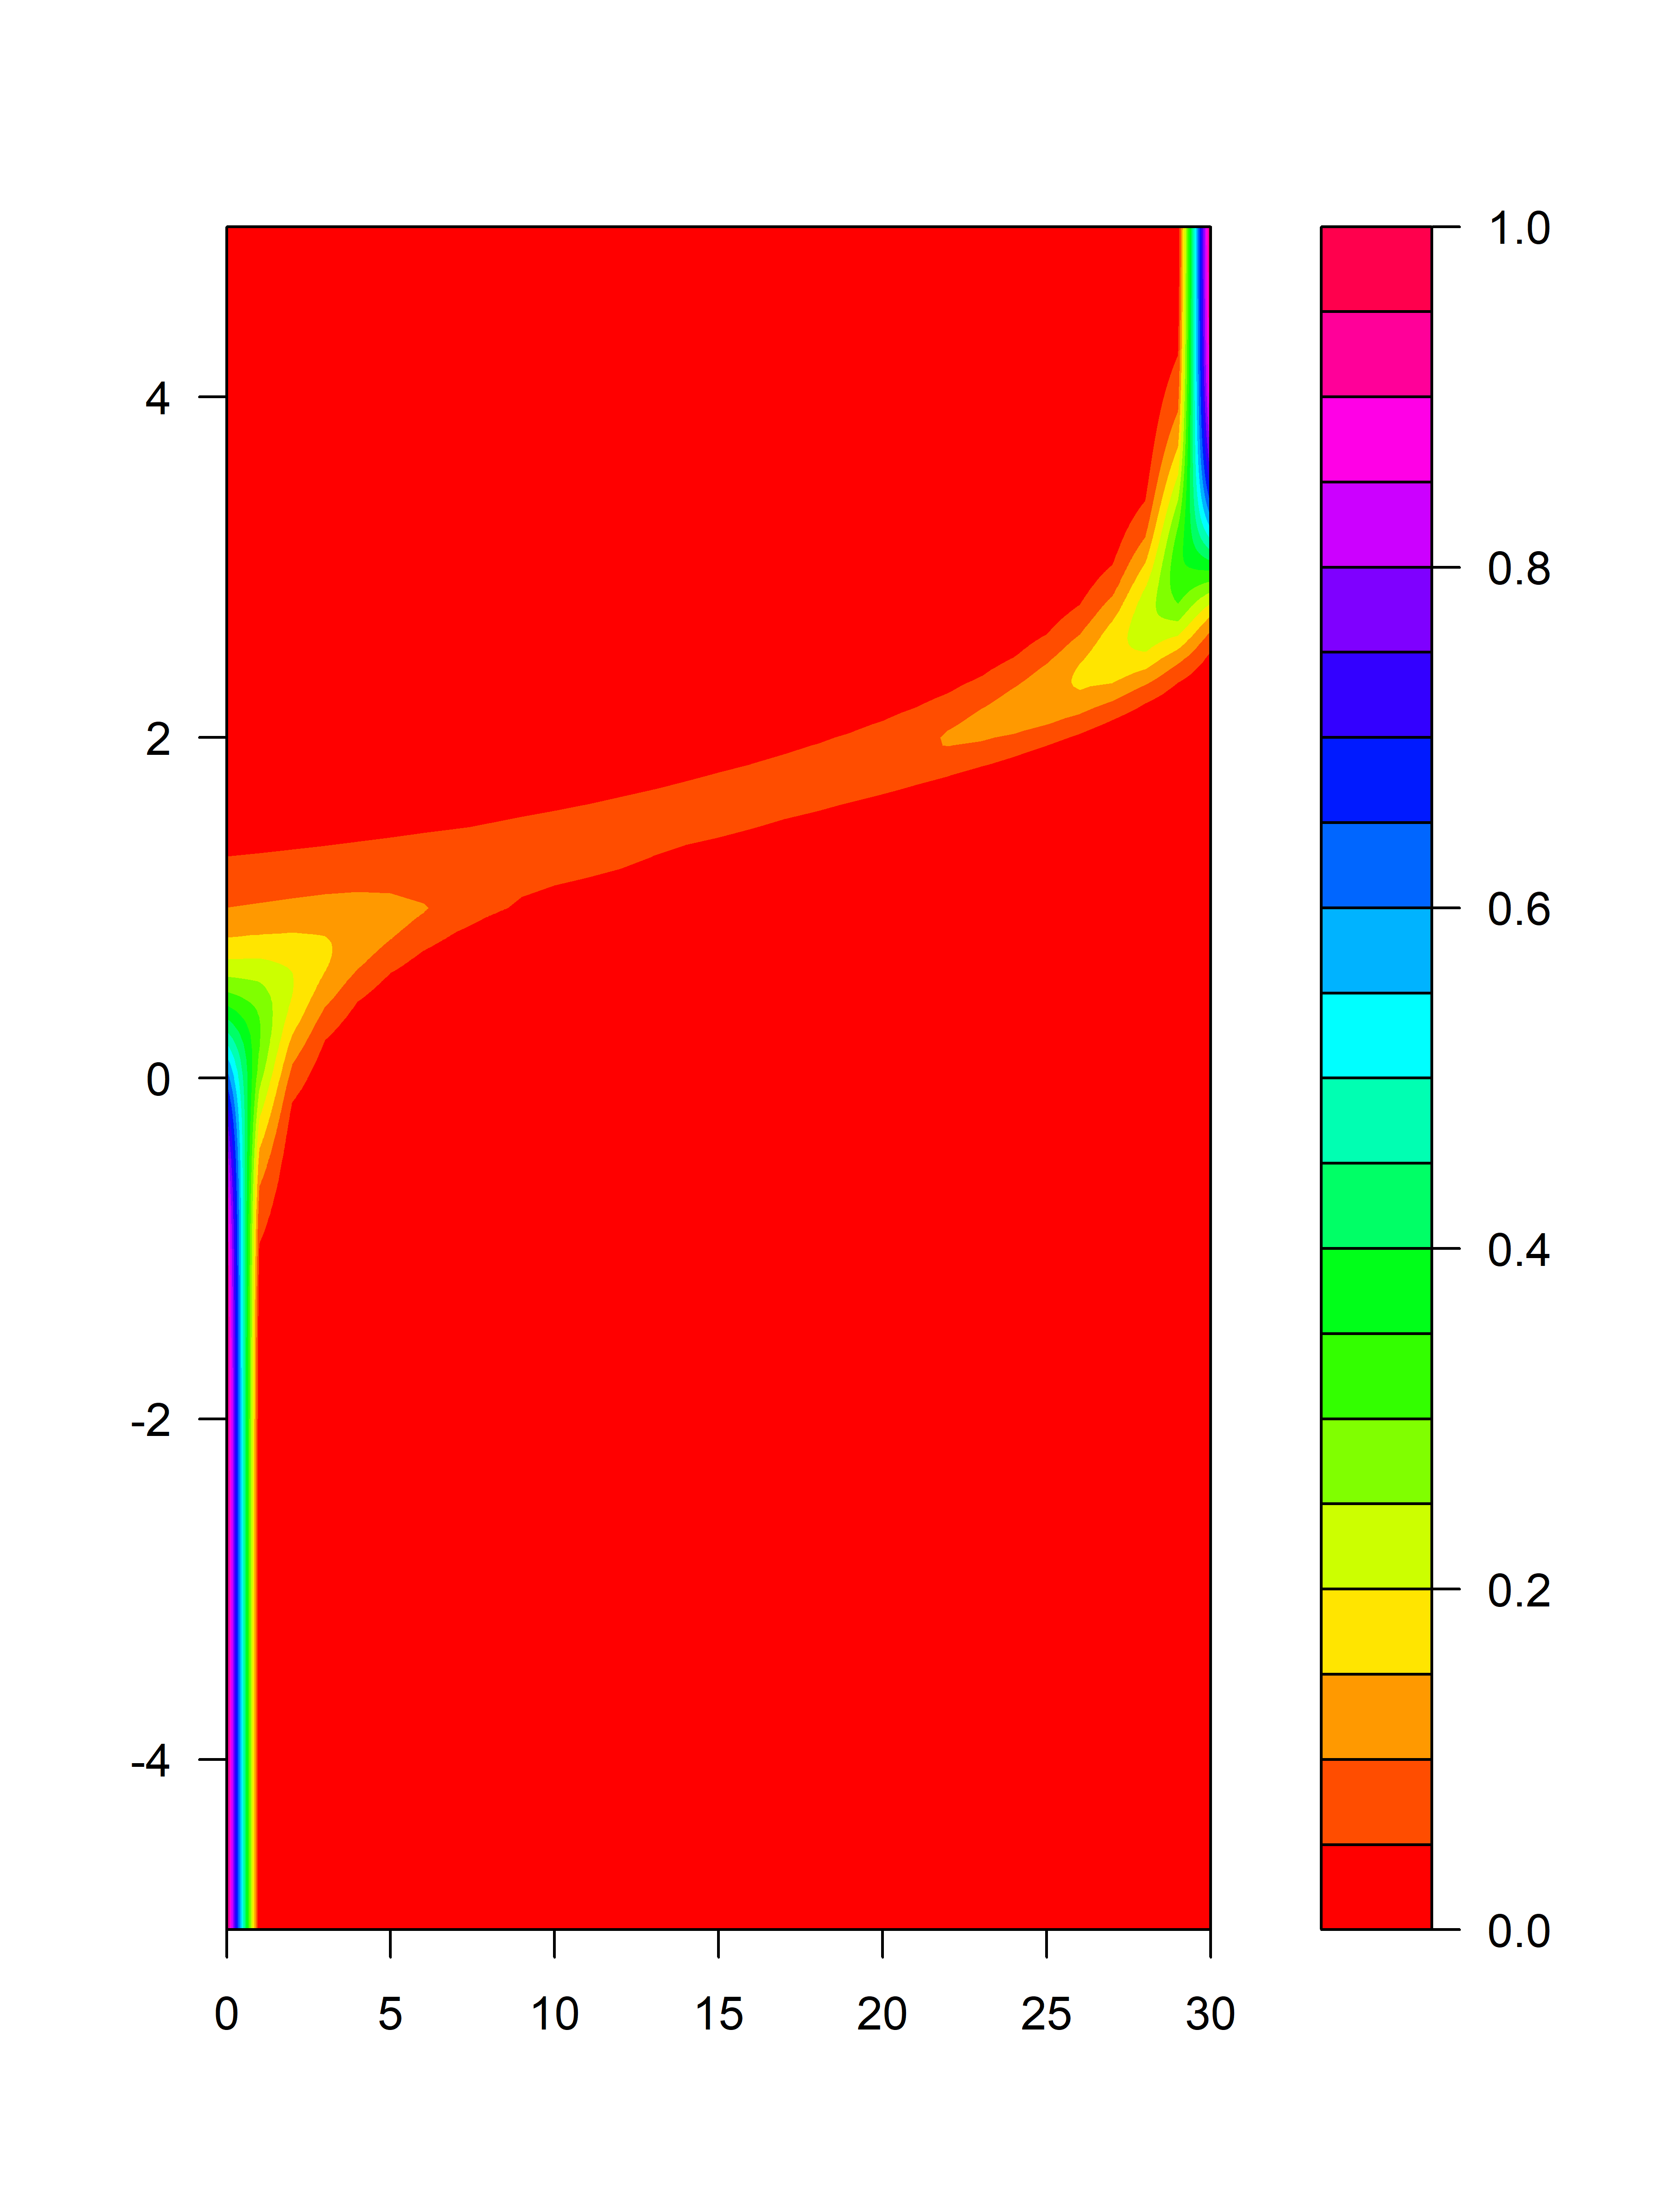
\includegraphics[width=30em]{Images/contour_norm_unmarked_l1m1d1t1_k1e-5_1e5_imax_30}
%		\caption{Contour plot of capped class over a range of kappa values: $\kappa = 10^-5 - 10^5.\imax=30,\lambda=1,\tau 0=1,\mu 0=0.1,\delta=100,000$. Color scale is percent ribomose load for each kappa value across all 31 ribosome classes.}
%		%\centering Red: decapped class, Green: capped class, Blue: Total= capped+decapped classes}
%	\end{figure}













%\begin{landscape}
%\begin{figure}
%\tiny
%\centering
%\caption{Equation~\ref{eq:matrix_capped}, $\vec{m}'=\bs{U}\vec{m}+\vec{b}$, is the matrix-vector equation representing the capped system from Section~\ref{sec:capped_simp}. As it can be seen, the matrix $\bs{U}$ is tri-diagonal, where all blank entries appearing in the matrix are 0. This property of $\bs{U}$ is desirable and leads to a scheme for finding equilibrium solutions that is presented later in this paper}
%\label{fig:capped_matrix}
%\[\left(\begin{array}{c}
%m_{0}'\\
%m_{1}'\\
%\vdots\\
%m_{i}'\\
%\vdots\\
%m_{\imax-1}'\\
%m_{\imax}'
%\end{array}\right)=\left(\begin{array}{cccccccc}
%-(\kappa_0+\mu_0) & \tau_0\frac{1}{\imax} &  &  &  &  &  &   \\
%\kappa_0 & -\left(\frac{\imax-1}{\imax} \kappa_0+\mu_0+\tau_0\frac{1}{\imax}\right) & \tau_0\frac{2}{\imax} &  &  &  &  &   \\
%   &\ddots        & \ddots        & \ddots & &  &  &  \\
%   & &    \frac{\imax-(i-1)}{\imax}\kappa_0 & -\left(\frac{\imax-i}{\imax}\kappa_0+\mu_0+\tau_0\frac{i}{\imax}\right) & \tau_0\frac{i+1}{\imax} &  &  & \\
%                  &         &        & \ddots  & \ddots & \ddots &  &   \\
%                  &         &        &  & \frac{2}{\imax}\kappa_0 & -\left(\frac{1}{\imax}\kappa_0+\mu_0+\tau_0\frac{\imax-1}{\imax}\right) & \tau_0\frac{\imax}{\imax} &   \\
%                          &        &  &  &  &  & \frac{1}{\imax}\kappa_0 & -\left(\mu_0+\tau_0\frac{\imax}{\imax}\right) \\
%\end{array}\right)\left(\begin{array}{c}
%m_{0}\\
%m_{1}\\
%\vdots\\
%m_{i}\\
%\vdots\\
%m_{\imax-1}\\
%m_{\imax}\end{array}\right)+\left(\begin{array}{c}
%\lambda\\
%0\\
%\vdots\\
%0\\
%\vdots\\
%0\\
%0
%\end{array}\right)
%\]
%\end{figure}
%\end{landscape}

%Include???

%From the matrix representation above, one can see that this system has a format, that when viewed in blocks, has desirable properties. Specifically the large square matrix $A\in\mathbb{M}_{2\imax+1,2\imax+1}$, is in the form where the upper-left block is tri-diagonal, and corresponds to the capped system. The lower left is diagonal, and corresponds to the input from the capped class to the decapped class, and the lower right is matrix is upper-triangular corresponding to the decapped system. There is an inhomogeneous term represented by the $\vec{B}$which functions as an input to the first capped class. These properties make it desirable to begin work by considering the capped and decapped classes separately.



%Units of the different paramters: $\lambda$ is transcripts/s, $\mu$, $\kappa$, $\tau$ and $\delta$ are is 1/s.

\subsection{model implementation in R}
Code to solve the model was written in the R package Ribosome. To solve the capped subsystem of the model, the Solve.tridiag routing from limSolve (Soetaert,K 2009). The model solutions presented previously serve their purpose to make the mathematics more interpretable by humans. However, solving for just the first column of the adjugate matrix is far slower than solving the whole tridiagonal system using limSolve. To solve for the deapped subsytem, the values of the capped state were plugged in to the solutions above. Utility functions, plots and statistics were created using R (v 3.6),  data.table (v1.14.0), and limSolve (v 1.5.6). 
		
\subsection{Data Sources}

In order to  interpret the model within biological context, we will focus on parameter ranges derived from the literature.
The range of \imax is determined from the distribution of protein lengths obtained from yeast (Figure 2A) or Arabidopsis (Figure 2C) which is then divided by the average number of codons covered by a ribosome (9 codons). 
Both were extracted from the Ensembl (version 109) and Ensembl plants (version 56) respectively (Cunningham 2022, Yates 2022, Kinsella 2011).  
The marking rate between the Capped and uncapped system was approximated from the protein half-lives from Presnyak 2015 for yeast (Figure 2B) and Sorenson 2018 for arabidopsis (Figure 2D).
 Presnyak utilized the temperature sensitive \textit{rbp-1} RNA polymerase mutant in yeast. This mutant can not undergo transcription at non-optimal temperatures, thus allowing for the measurement of mRNA decay over time. Sorenson (2018) used the transcriptional inhibitor, cordycepin, to treat  \textit{Arabidopsis thaliana} seedlings and measured their decay using RNA-Seq.
To approximate $\mu$ transcript half-lives were converted to rates with the following:
	\begin{equation}\label{eq:eq_half-life_conversion_to_rate}
		\mu = \frac{ln(2)}{t_{1/2}}
	\end{equation}
Where $t_{1/2}$ is the half-life. The resulting range of $\mu$ is from $10^-2$ to $10^-4$ for yeast and $10^-3$ to $10^-6$ for arabidopsis. 

Translation initiation and elongation rates ($\kappa$ and $\tau*9*\imax$) were obtained for Yeast from Duc and Song 2018. Remember, that $\tau$ is the overall rate of translating a transcript, not the average elongation rate (see section 2.2). In Duc and So stng 2018, the authors used 850 highly translated transcripts from the ribo-seq dataset from Weinberg 2016. They employed a TASEP model to estimate the initiation rates and correct the empirical elongation rates from the footprint distributions. We calculated an average gene specific elongation rate from the corrected elongations rates. We scale the each gene specific initiation rate by dividing it by the gene specific elongation rate.This is due to the fact that many combinations of $\kappa$ and $\tau$ can yield the same scaled initiation rate (e.g. $\kappa$ =0.02 and $\tau*9*\imax$ = 2, and $\kappa$=0.04 and $\tau*9*\imax$=4, both yield $\kappa/\tau$=0.01). This simplifies the model behavior to one generalized parameter with a unique response (Figure 2E).  The scaled initiation rate ranges from 0.1$s^{-1}$ to 0.001$s^{-1}$.

The transcription rate, $\lambda$ only acts as a scaling factor throughout the model and does not affect the distribution of the ribosomes. For solutions provided in this work $\lambda$ has been set to one. However, as a point of reference, the transcriptomic results from Weinberg 2016 are included in Figure 2F. In short, reads per kilobase million from Weinberg were further converted into a log10 fold change based on the median expression level. Figure 2F shows that the absolute range of transcriptional control ranges just under 5 orders of magnitude.

Finally, $\delta$ only determines the accumulation of transcripts in the  $m_0^*$  class. In our model the remaining transcripts in class $m_0^*$ are either only the 3' end of co-translationally degraded transcripts or full transcripts from class $m_0$. Recently, the rate of degradation for the 5' - 3' exonuclease XRN1 was determined to be ~26 nt/s (Atthapattu 2021). XRN1 is the primary exonuclease involved in co-translational degradation and  5' degradation pathways (Sorenson 2018,Yu 2016, Collart 2019, Pelechano 2015). For an average 3' UTR of 121 nts (Kebaara 2009) this would take ~4.6s, and an average transcript of ~ 1400nt would take 54s to degrade.  This means the average degradation rate $\delta$ would take between 1/54s = 0.019/s or 1/4.6s = 0.22/s . The total population of mRNA in $m_tot^*$ is determined by $1/\delta$, $1/\tau$ and $\mu$ (as part of $\vec{S}$) as shown Equation  ~\ref{eq:  marked_total_pop}. $\tau$ ranges from 0.03 to $10^-4$. This makes $1/\delta \leq 1/\tau$. It is reasonable to explore the model with large $\delta$ since decapped transcripts are translationally incompetent. 
 
\begin{figure}[!ht]
\centering
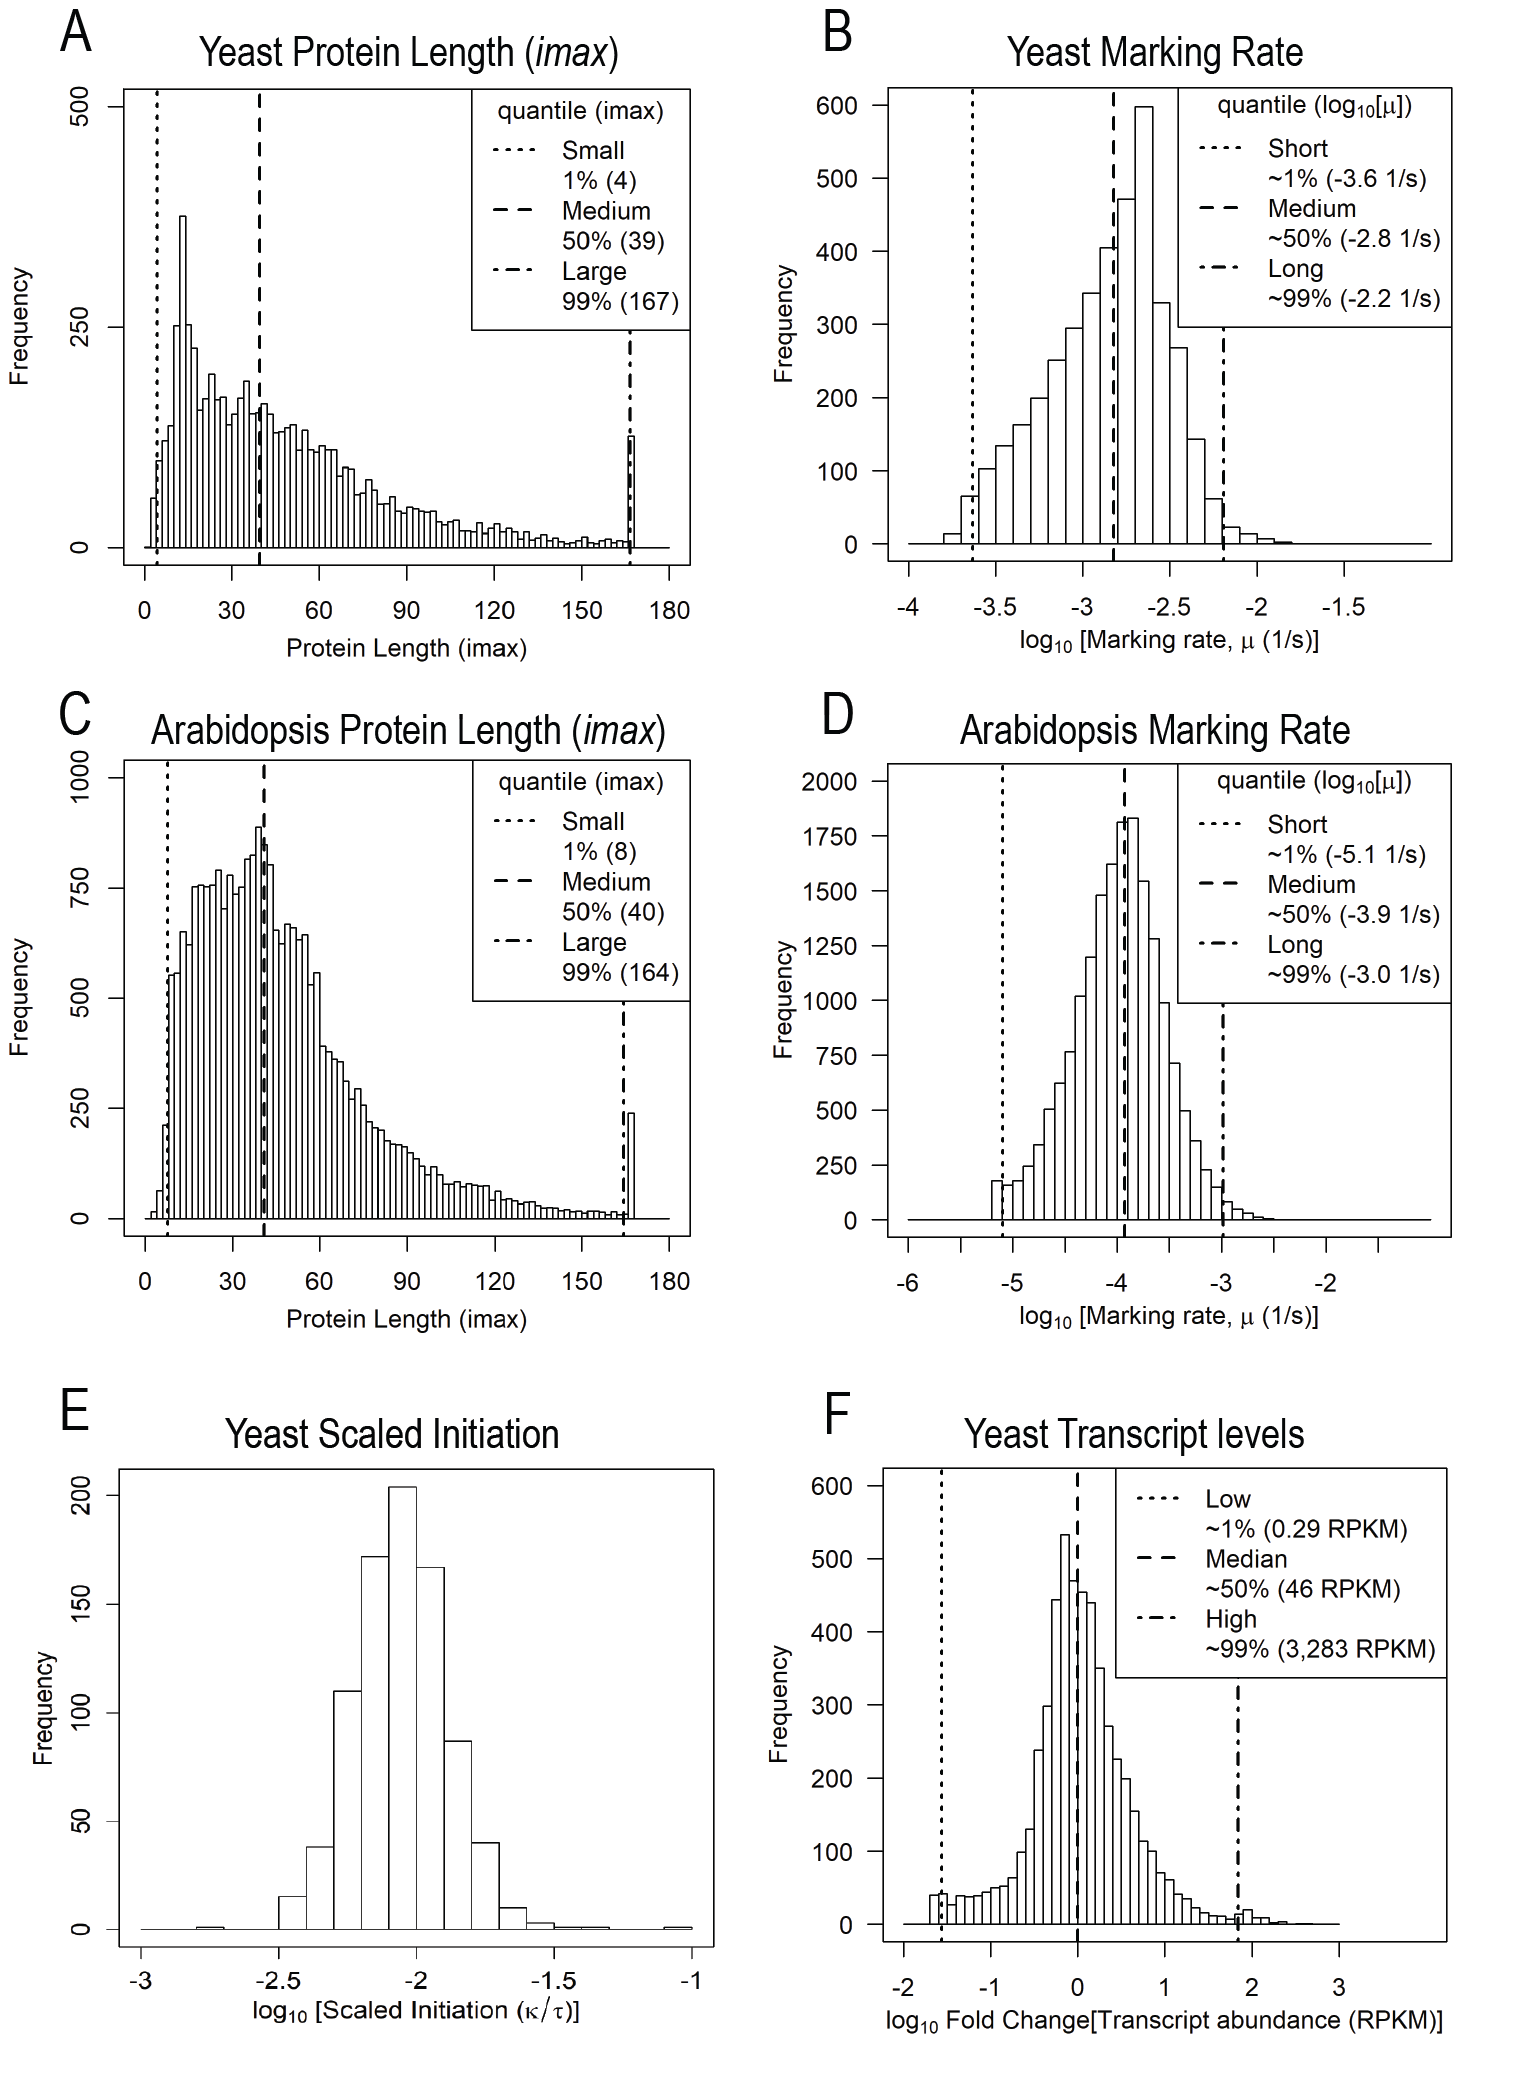
\includegraphics[width=120mm]{Images/2023-07-04_parameter_histograms.png}
\caption{Histograms of empirical values of model parameters. A) Yeast protein lengths. B) Yeast half-life C) Arabidopsis Protein Lengths. D) Arabidopsis Half-Life. E) Yeast Scaled elongation rates (Translational initiation rate/average translation elongation rate) on a per gene basis. F) Log 10 Fold Changes between all transcripts compared ot the median transcript expression in yeast. }
%\centering Red: de_s class, Green: capped class, Blue: Total= capped+decapped classes}
\end{figure}
		


% It could be futher extended to include more degradations mechanisms see note below
% $\delta\ might be more complex with a slightly different model design. In the current model formulation it mimics the primary (but not only) degradation with the cell, the 5' decapping and subsequent VCS /XRN1 5'-3' cotranslation degradation system. This ignores 3 other systems the two 3'- 5' pathways (CCR4-NOT3) and exosome, and the final slew of endodegradation pathways (NGD, NSD, NMD, ribothrypsis, and silencing).
%Additionally, degradation of the bulk of the mRNA transcript might not be a process specific to each transcript (ie. due to coding sequence, I would have to look this up. Also might be testable with data fitting).


\section{Results}

The model outputs two sets of results. First it provides the total mRNA population and how this population is split between capped and decapped states. Secondly, it describes how transcripts are distributed among ribosomal classes within each state. 

\subsection{Marking rate and ribosomal load determine mRNA distribution between states}

%Main results: 
%Link our mean output and the results of TASEP ribosome flow model.
%because short genes experience inteference at short loads becomes accentuated because turnover rate is high
%mention heterologous expression due to codon usage bias
% mean initiation rate to mean elongation rate ratio and shorten it to the Initiation elongation ratio 

%Point for discussion. By varying the granularity of the Ribo flow model it would be possible to fit the model for distinct regulatory regions. In this idea I'm trying to communicate that there might be distinct mRNA regions that behave like different transcripts. Some transcripts might be very granular like every 10 codons has a distinct behavior, But i would imagine that any one major bottleneck in a transcript would make it

\begin{figure}[ht]
\centering
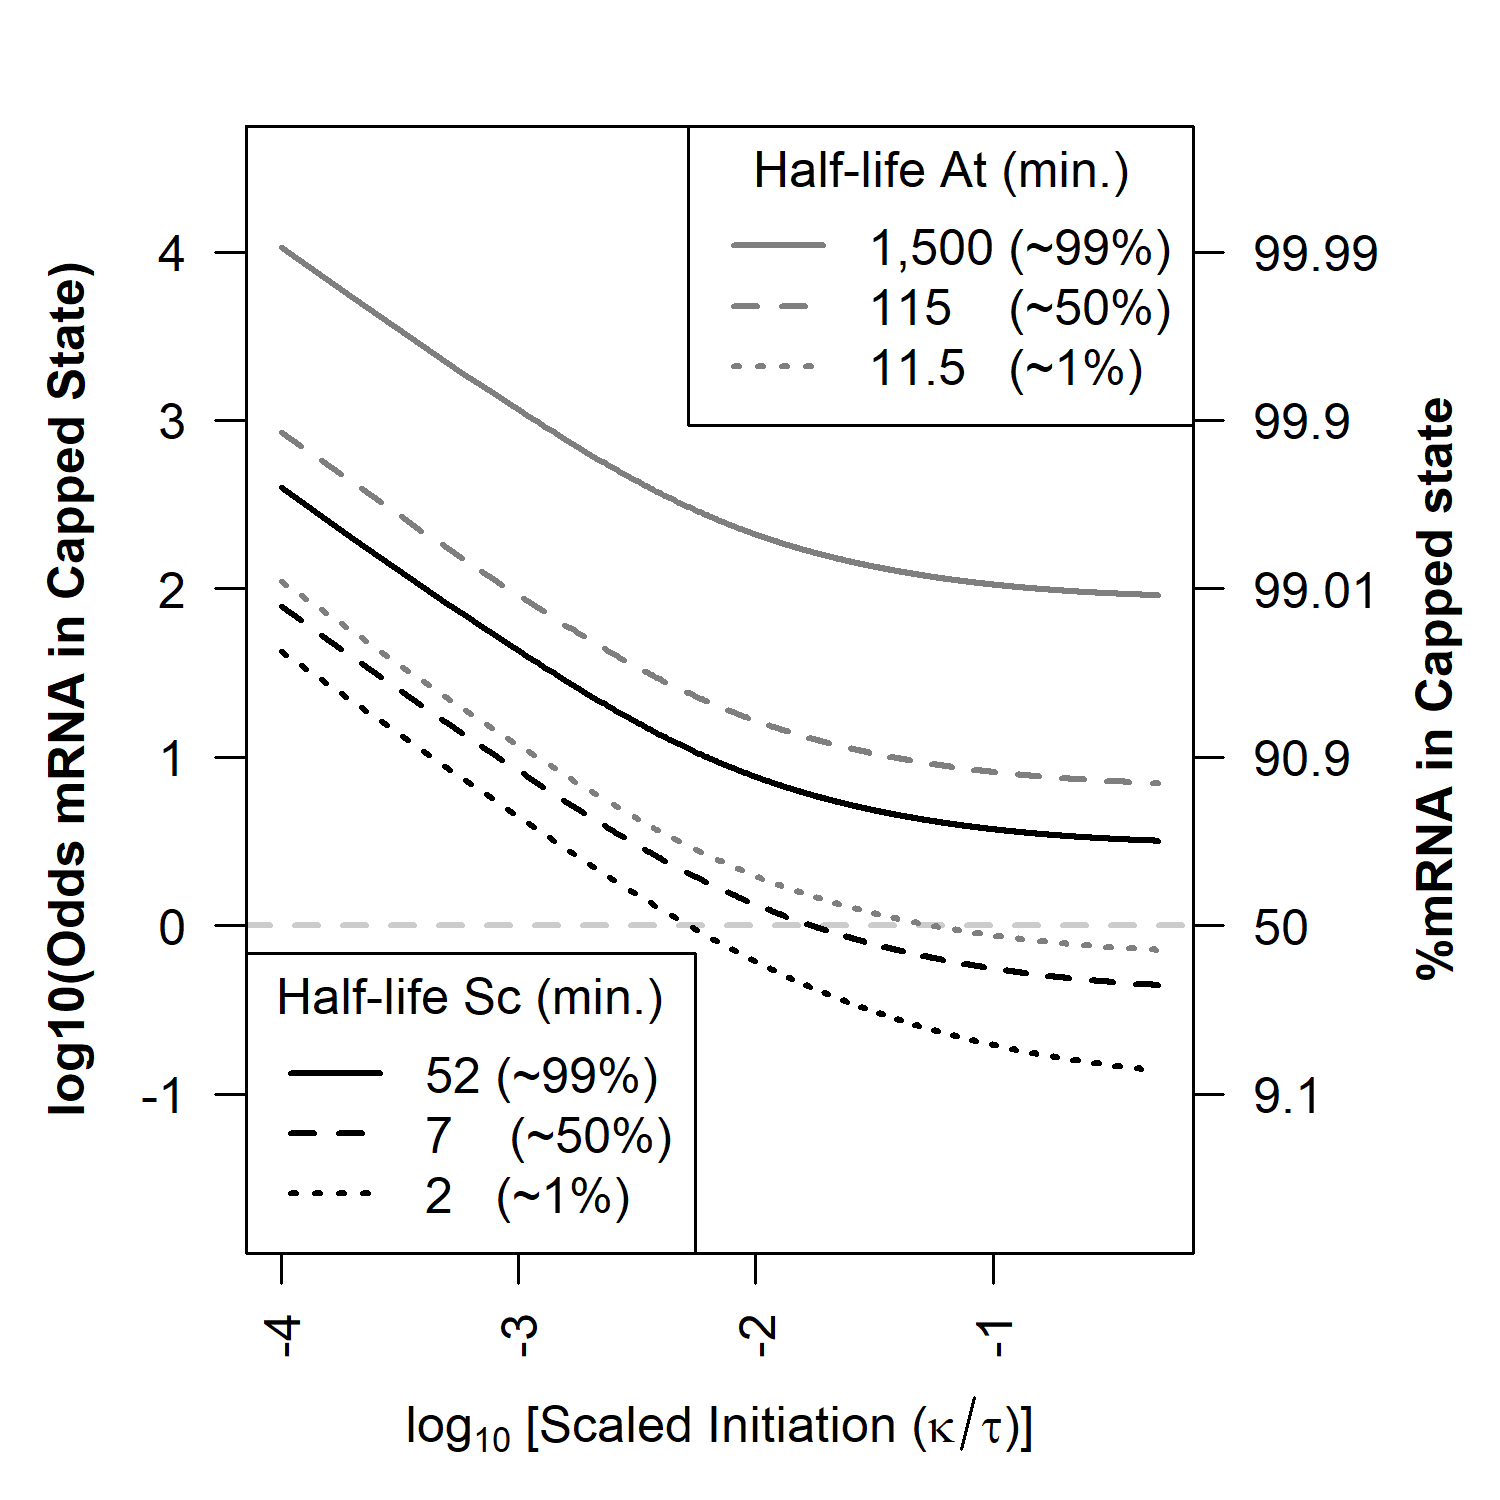
\includegraphics[width=100mm]{Images/2023-07-02_logodds.png}
\caption{Log odds of finding mRNA in the capped state for a range of marking rates in yeast and arabidopsis. }
%\centering Red: decapped class, Green: capped class, Blue: Total= capped+decapped classes}
\end{figure}




\begin{figure}[ht]
\centering
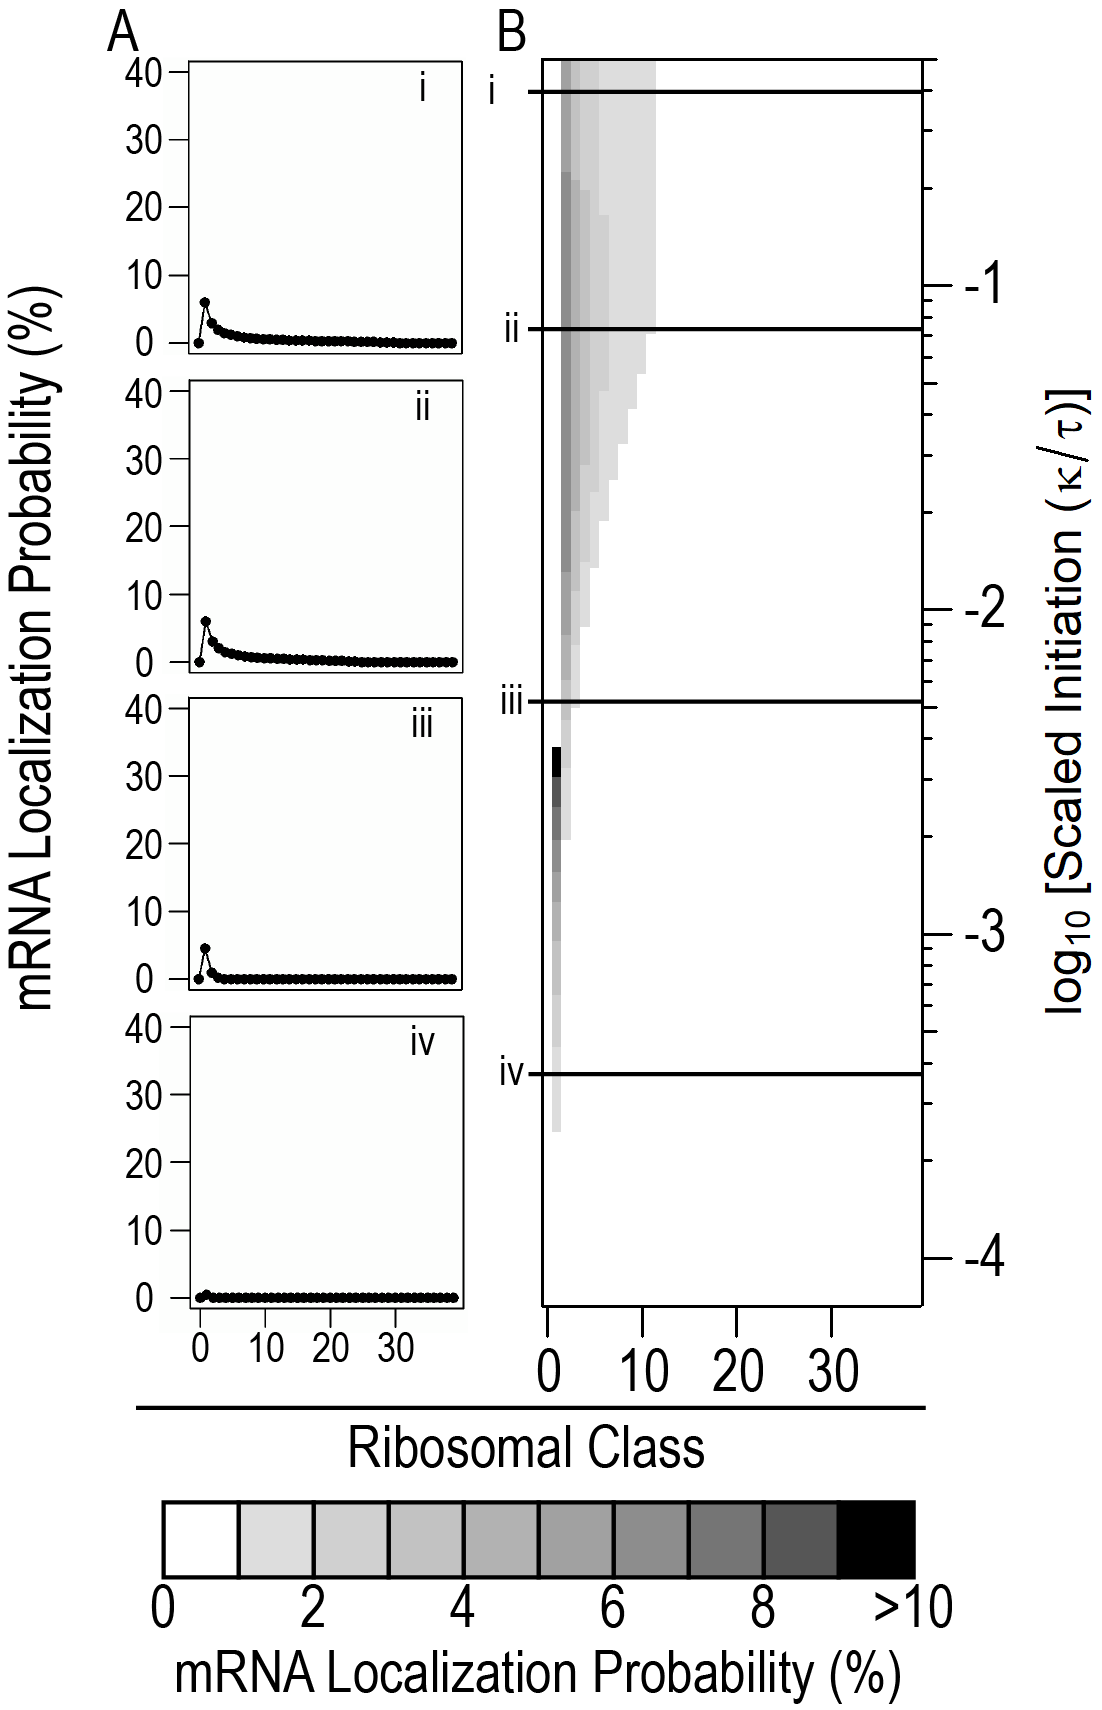
\includegraphics[width=100mm]{Images/2023-07-04_Marked_slices.png}
\caption{Comparison of density independent initiation (DII) and density dependent initiation (DDI)}
%\centering Red: decapped class, Green: capped class, Blue: Total= capped+decapped classes}
\end{figure}



Supplemental Figure 1
\begin{enumerate}
	\item The model solution at equilibrium has three outputs.
	\item First the total number of mRNA transcripts.  Second split between the capped and decapped states. And third the distribution of the transcripts across ribosomal classes for each of the states.
	\item  s

	\item After exploring the model solutions it was determined that the transcription rate $\lambda$ acts simply as a scalar for the whole system. 

\end{enumerate}


\begin{figure}[ht]
\centering
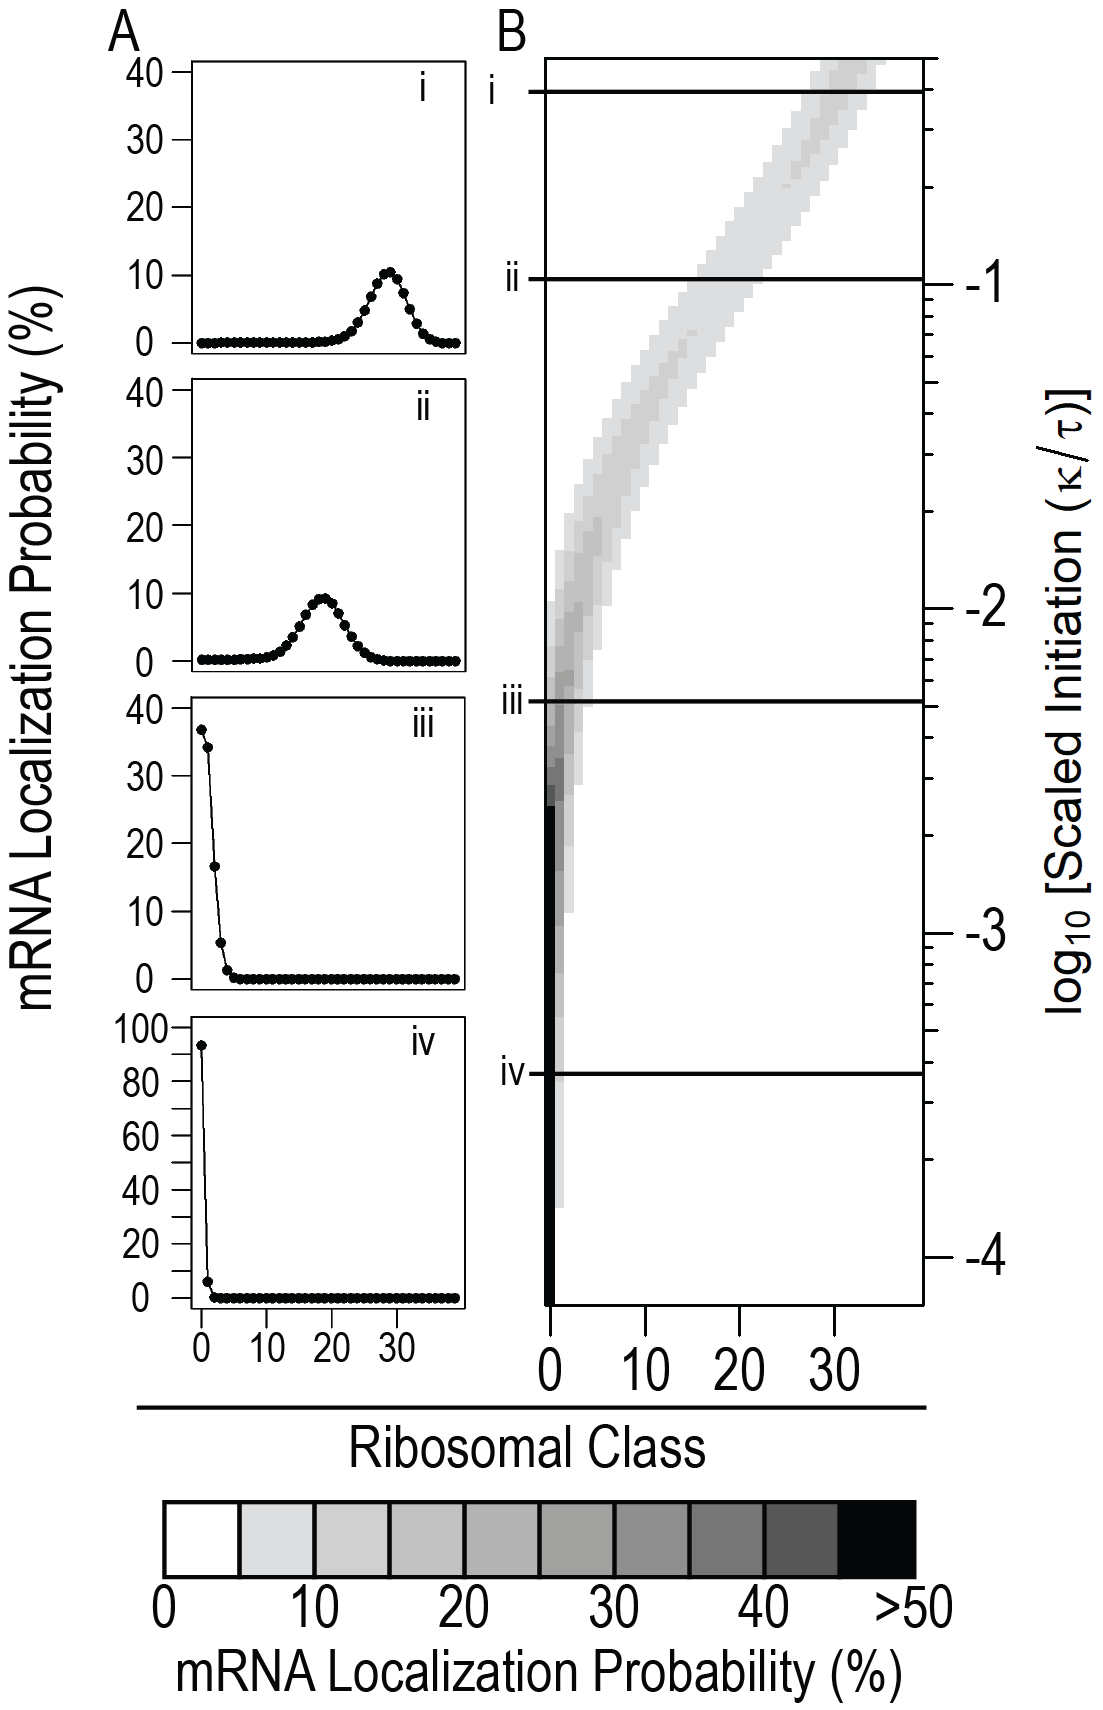
\includegraphics[width=100mm]{Images/2023-07-04_Unmarked_slices.png}
\caption{Comparison of density independent initiation (DII) and density dependent initiation (DDI)}
%\centering Red: decapped class, Green: capped class, Blue: Total= capped+decapped classes}
\end{figure}

Text for discussion of figure 1
\begin{enumerate}
	\item The model presented most closely resembles the co-translational decay pathway from eukaryotes.
	\item There are a few current limitations of the model. First and foremost it doesn't model endonucleolytic decay pathways such as gene silencing by siRNA and the RISC complex or the NMD, NGD and NSD pathways or degradation initiated through ribosomal collisions.
	\item Implementation of endonucleolytic decay would require an ability to track ribosomal position, which is not possible in our model. 
	\item Alternatively a probabilistic model of ribsomal position given a particular load could allow for redistribution of capped transcripts into decapped states of lower ribosomal class.
	
	\item Currently there is a debate whether mRNA stability is regulated primarily through the protective effects of ribosomal association or through the suboptimal codons causing ribosomal stalling and the subsequect ribosome associated decay pathways  (Chan elife).
	\item We explored the interaction of ribosomal loading and marking rate, noting that increased marking leads to a lower expected ribosomal load. This particularly noticable for genes with short half lives and is less sensitive with transcripts with halflives above 2 hours.
	\item In the current implementation of the model we did not directly explore the protective effects of ribosomal loading. This could be first implemented by including a similar weighting term analogous to the wieght for the intiation rate of (1-i/imax).
	\item However, biology suggests a more complex behavior.
	\item The protective effects of translation could increase per ribosome, but eventually at high loads  could trigger ribosome associated decay pathways through ribosomal collisions.

	\item Our model does not model elongation at a single codon level like TASEP, nor at a course grained approximation of groups of codons like the ribo flow models. This means that it is not capable of analyzing the effect of individual non optimal codons, or stretches of mRNA which are non-optimal
	\item Our model reflects the average elongation rate over a transcript. However it can be set to reflect the slowest bottle neck across a transcript.  
	\item Another alternative to modeling bottlenecks is increasing granularity to a very coarse grained ribo-flow model comprising of only two or three sectors, depending whether the transcript has one or two bottlenecks. 
	\item This splits transcripts into an intial sections where the bottleneck effectively "shortens" the transcript length to the first bottleneck site. Increasing the effect of ribosome loading on iinitiation interference. 
	\item However, the transcript physically has more length and can bear a larger ribosomal load on the section section. This results in a transcript having and "effective" imax between the actual coding sequence length and the lenght of the transcript to the first bottleneck. 

\end{enumerate}

	Model predicts mRNA distribution across ribosomal classes
	\begin{enumerate}
		\item The model 
		\item Density independent initiation and density independent initiation models
		\item The model predicts the steady state total mRNA quantity in both decapped and capped states as well as the mRNA's distribution across different ribosomal classes in each state.
		\item  Figure X Left, 
	\end{enumerate}
	The model provides an upper bound on translational efficiency
	\begin{enumerate}
		\item  The behavior of both DDI and DII models were explored at equilibrium.  At equilibrium, the rate of new initiation events must be equal to the rate of ribosomes leaving the transcript. 
		\item The two key parameters that control this process are initiation ($\kappa$) and elongation ($\tau$). Changes in either parameter alter the predicted distribution of transcripts across ribosomal classes. 
		\item To summarize their joint behavior, we chose to focus on the elongation scaled initiation rate ($\kappa$$\\$$\tau$) as this provides a single unique parameter for each model response. %Elaborate on how this is unique and why this is important. This is a necessary reduction of the parameter space that can then be reverted with knowledge of the elongation rate from codon usage data or from ribo seq
		\item  Exploration of the steady state solution showed that the transcription rate only acts to scale the steady state solution. Meaning that the distribution of transcripts across the ribosomal classes is independent of the number of transcripts being produced. All model solutions presented here have the same transcription rate to allow for comparison. 
		\item The degradation rate ($\delta$) only controls the transcript population in the decapped zeroth class. To reduce interference from this we set a very high degradation rate.
		\item To interpret model behavior within a biologically meaningful context, empirically determined rates for translation initiation, elongation, and half-life (as a proxy for marking rate) were obtained from the literature. 
%		\item First, average initiation rates in yeast had an average of 0.131 initiation events/s (5th percentile: 0.07 events/s, 95th percentile: 0.26 events/s) . Paired elongation rates for individual genes were not available. However, empirical elongation rates for each codon from the same experiments were available. A weighted average of elongation rates across all protein coding codons (weighted on the codons abundance) gave a mean elongation rate in yeast. The distribution of elongation values was produced using the weighted mean and the average standard deviation of all codons resulting in a mean elongation rate of 5aa/s (5th percentile: 1 aa/s, 95th percentile: 9 aa/s) [31]. The resulting scaled initiation rate ranges from 0.001 to 0.261. This is old. I have since found a different paper which uses the ribo flow model in yeast to estimate the scaled initiation (Duc 2018)

		\item Introduce scaled initiation rate range. Discuss upper and lower limits vis a vis the model output. 
		\item *** This is a very important question. How do we show in a convincing manner that the model is recapitulating actual biological results? I have previously used the arguement that both polysome profiling and single molecule imaging of in-vivo ribosomes all agree with the approximate range predicted by the model, especially within the scaled initiation values. That is the model predicts that the ribosome load will be between 10-50$\%0$, with median loads of 2 - 13 ribosomes for a transcript of median length. This is reasonable and the median behavior aligns with what polysome profiles show. However, Polysome profiles contain all of the mRNAs in a cell or organism at once. This means that the fact that the model predic 

(-3 to -0.6 in log ten). The marking rate was determined from Arabidopsis mRNA half-lives with a median half-life of 115 min (short 1st percentile: 11.5 min, long 99th percentile: 1,500 min) [32]
To establish the base model behavior, DII and DDI models were run with a long half-life across a broad range of scaled initiation on a transcript encoding a protein of median length (369aa) (Figure 1). In the DII model, all ribosomal classes are populated. At the high end of the biological scaled initiation transcripts reach full ribosomal occupancy (Figure 1A). The DII model ignores initiation interference caused by ribosomes already present on the transcript. The DDI model accounts for initiation interference, and as expected, a decrease in ribosomal load is observed compared to DII. Even with interference, access to most ribosomal classes is attainable in the DDI model. Ribosomal profiling experiments suggest that most transcripts have one to ten ribosomes loaded with a strong preference for smaller polysomes. Live single molecule fluorescence experiments do show higher polysome numbers rising into the 50s [33]. For the long reporters used in these experiments that equates to a 12 to 30 percent ribosomal load. Thus the DDI model probably overestimates the loading for a particular scaled initiation rate.
	\end{enumerate}
	Marking rates have only a mild effect on ribosomal load, but a large effect on protein production.
	\begin{enumerate}
		\item From the solution of the capped system we can define two separate effects of transcript marking.
		\begin{enumerate}
			\item  First, marking determines how many transcripts can accummulate in the capped class, thus determining the total transcript population		
			\item Second, marking rate shifts the distribution of transcripts  in the capped class towards lower ribosomal classes.	
		\end{enumerate}
		\item Marking only has a mild effect on the distribution of transcripts on the capped class


	\end{enumerate}
	Under equilibrium protein length affects ribosomal load but not ribosomal density
	\begin{enumerate}
		\item stuff
	\end{enumerate}



Figure 2 points for discussion

\begin{enumerate}
	\item

\end{enumerate}



\begin{figure}[ht]
\centering
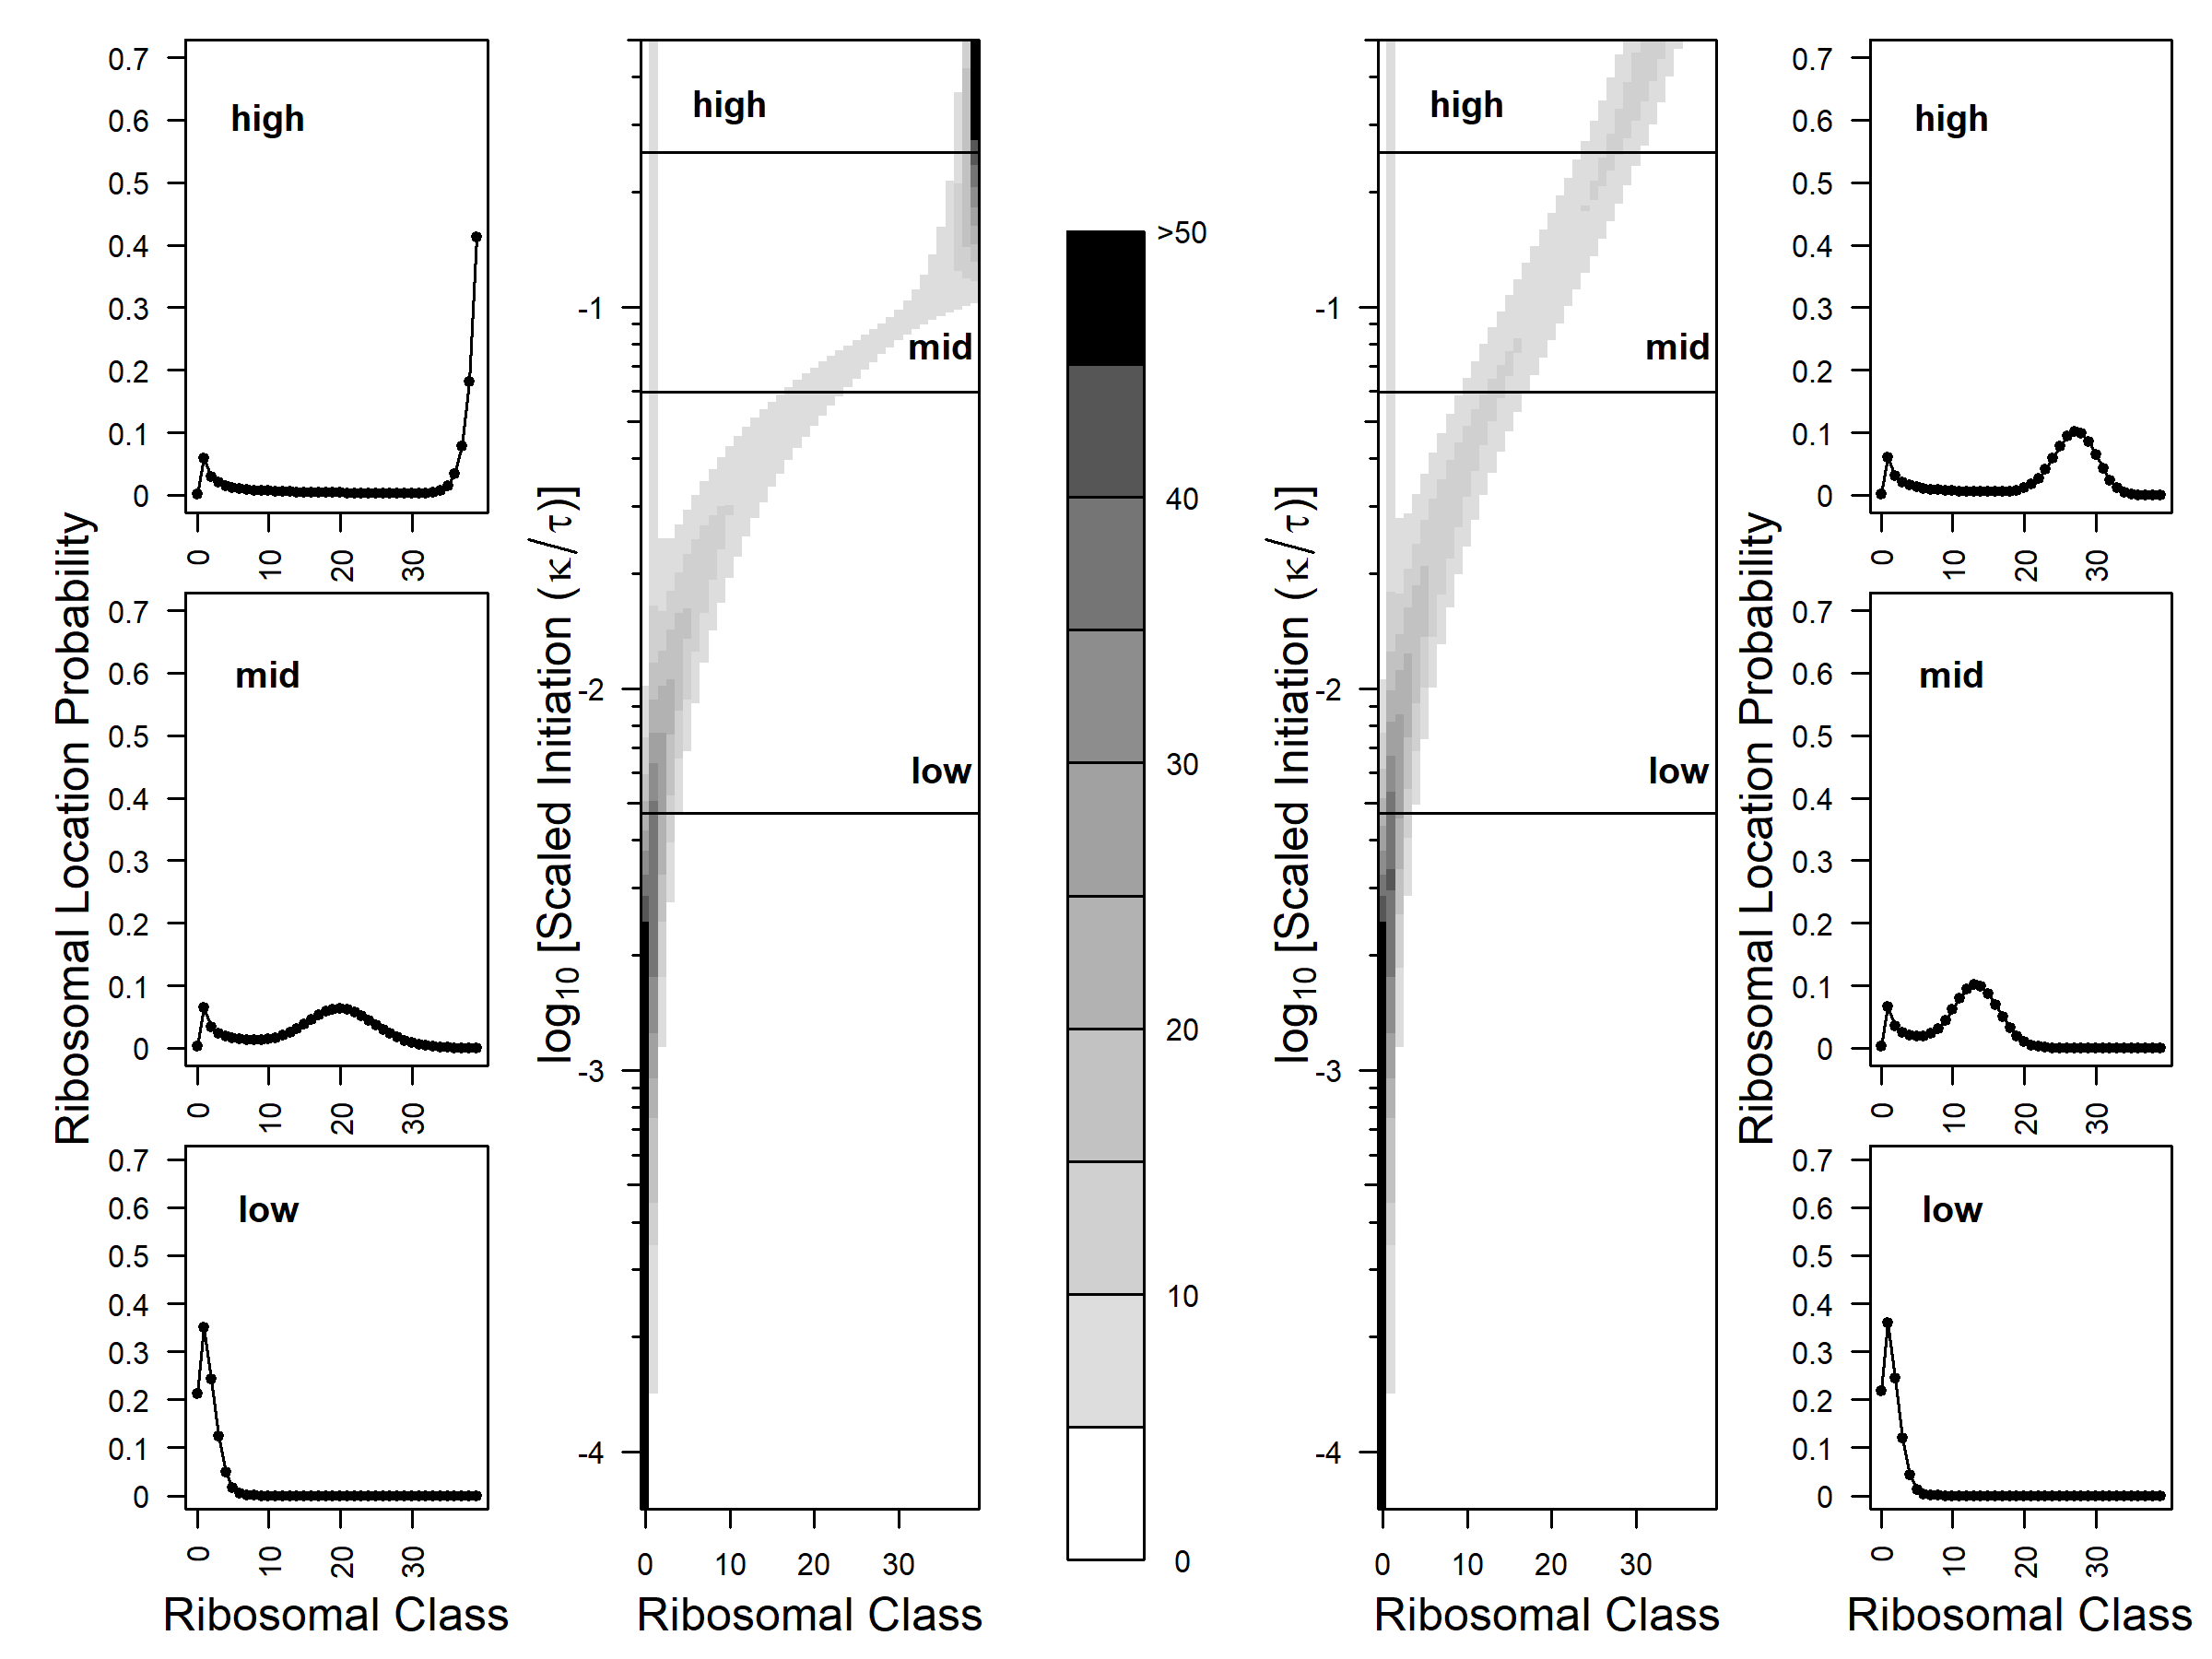
\includegraphics[width=150mm]{Images/2023-06-28_Figure1_DIIvsDDI_medianlength_low_marking.png}
\caption{Comparison of density independent initiation (DII) and density dependent initiation (DDI)}
%\centering Red: decapped class, Green: capped class, Blue: Total= capped+decapped classes}
\end{figure}


\begin{figure}[ht]
\centering
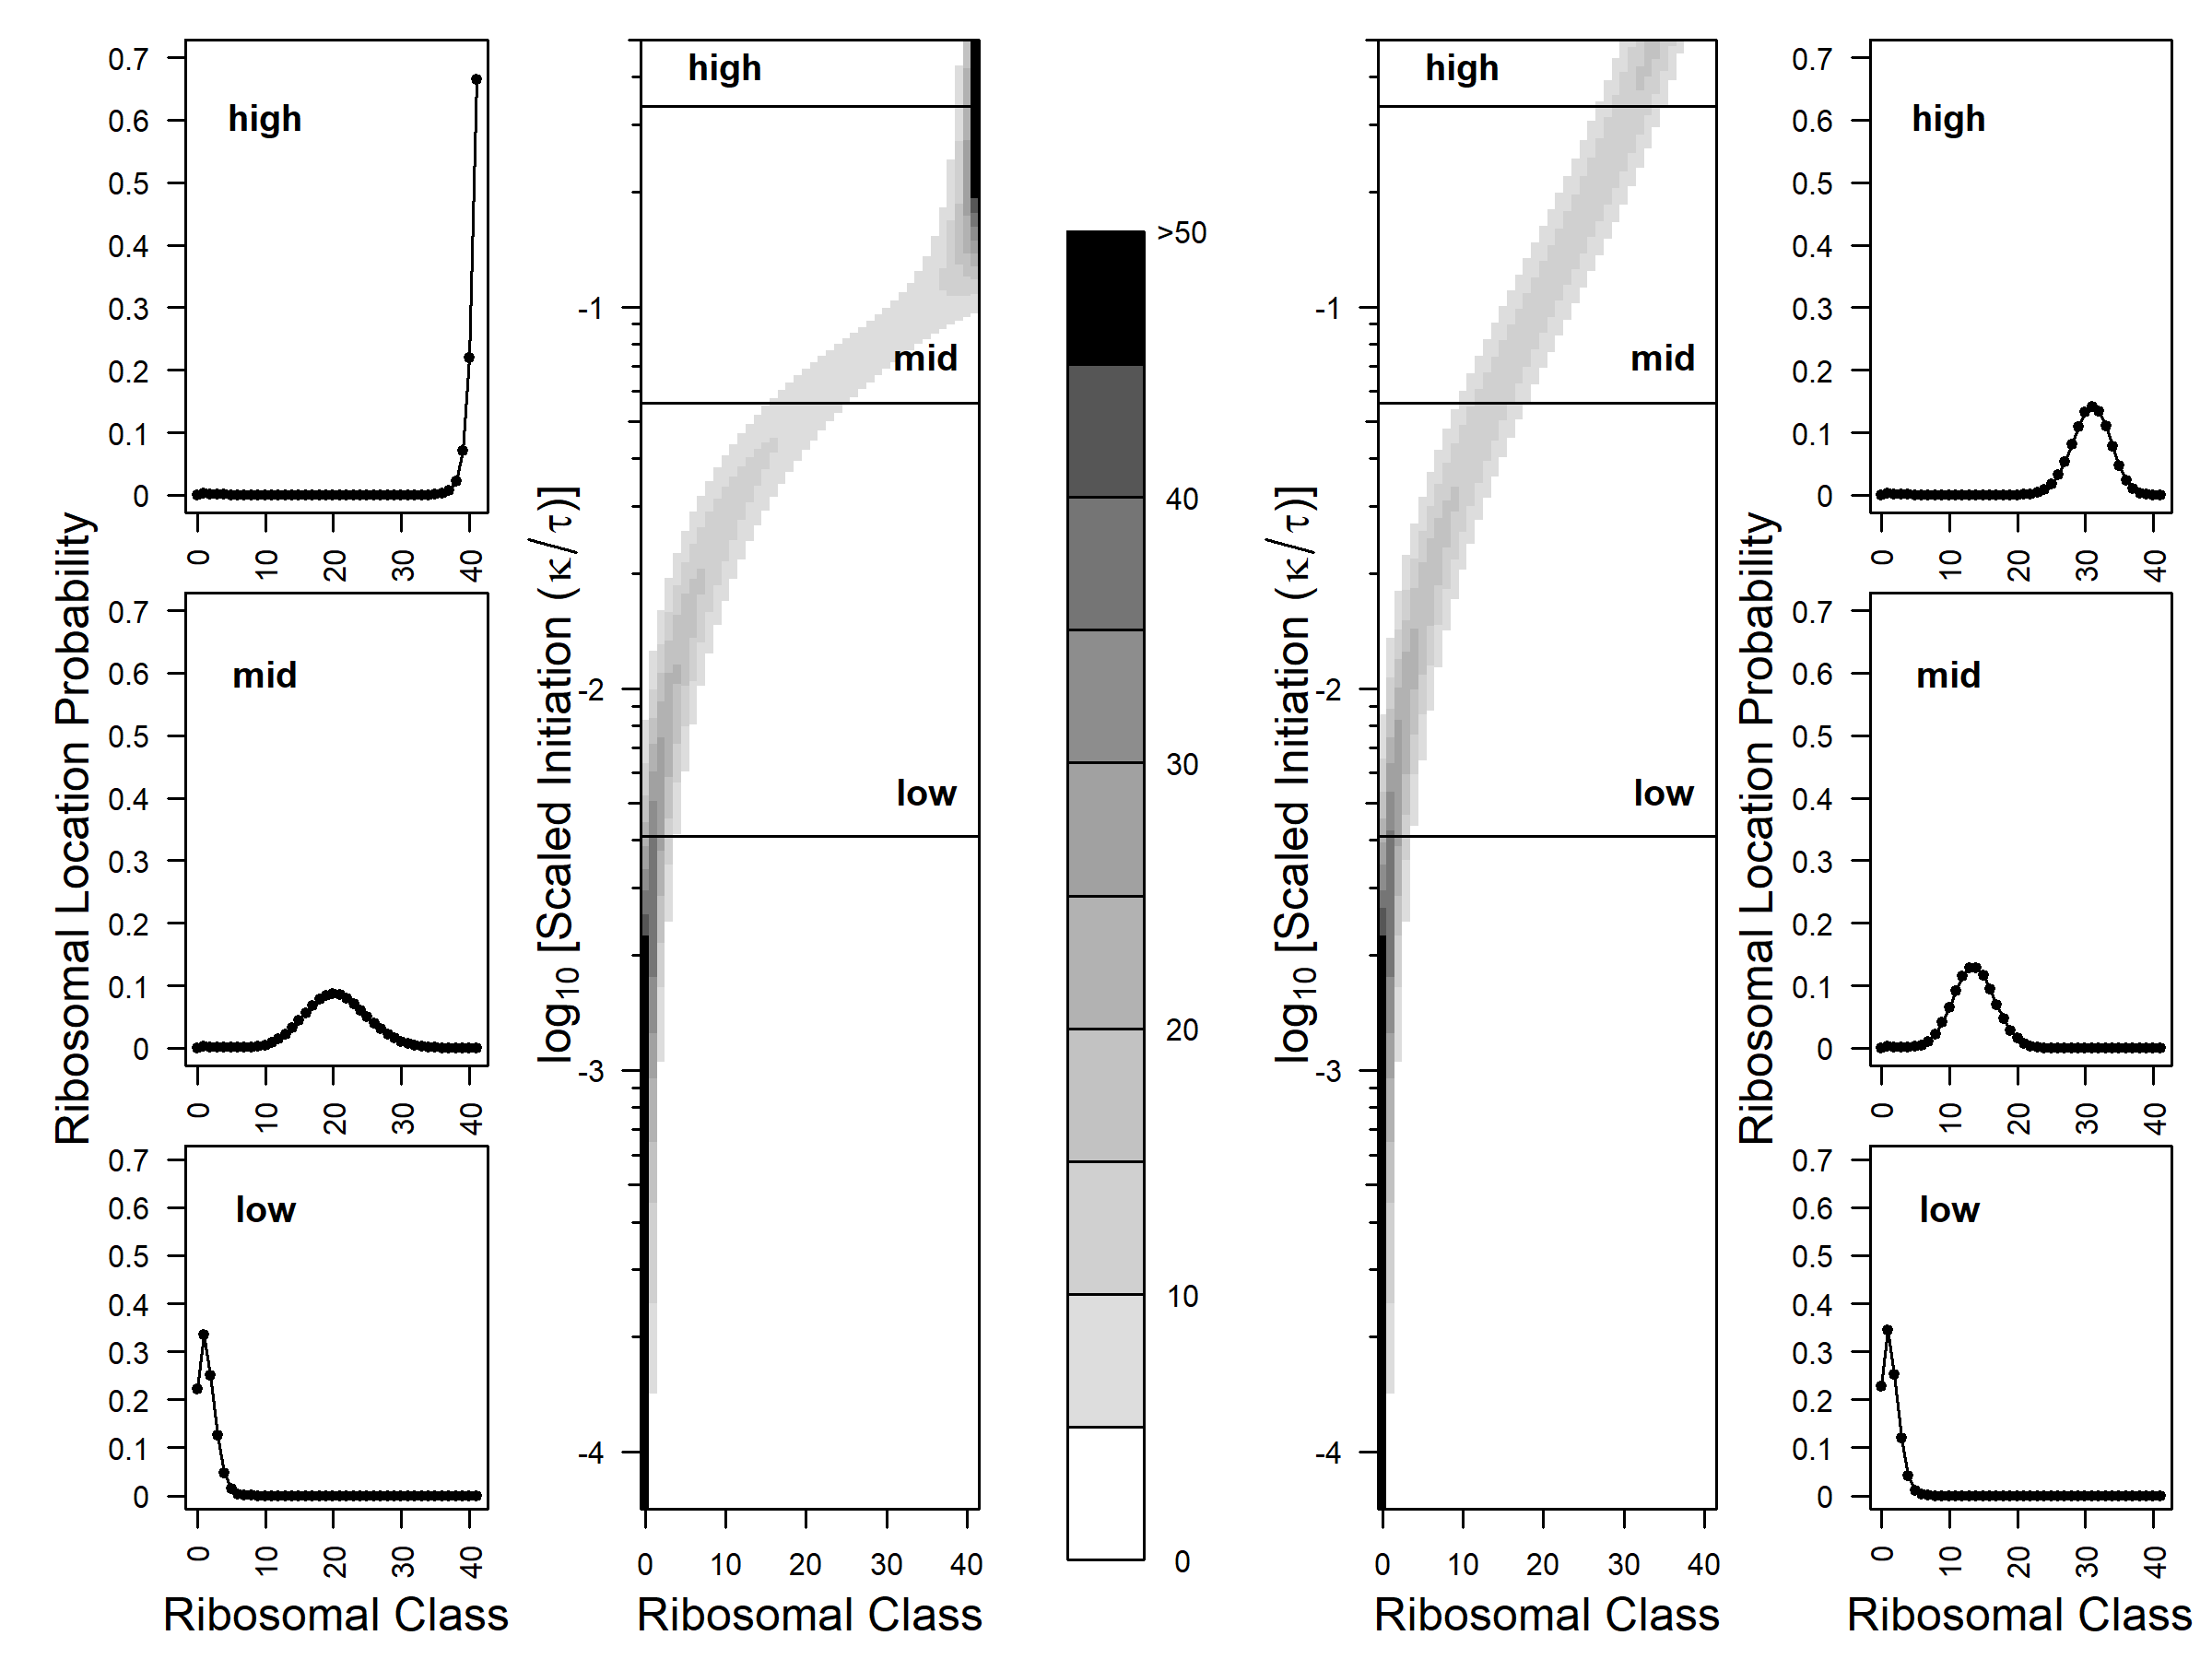
\includegraphics[width=150mm]{Images/2022-10-21_Figure1_DIIvsDDI_medianlength_low_marking.png}
\caption{Comparison of density independent initiation (DII) and density dependent initiation (DDI)}
%\centering Red: decapped class, Green: capped class, Blue: Total= capped+decapped classes}
\end{figure}


\begin{enumerate}
	\item  As more ribosomes are loaded onto a transcript there is reduced space available for new ribosomes to occupy.
	\item This in turn would reduce the ability to initiate new rounds of translation.
	\item To investigate the effect of ribosomal density on initiation we created two versions of the model. A density dependent initiation (DDI) model which scales the initiation rate by the number of ribosomes on the transcript. And a density intedpendent initiation (DII) version of the model which has a fixed initiation rate.
	\item In the DII model the ribosome load increases linearly with the scaled initiation rate ($\kappa$ \ $\tau$ ) until it reaches 
	\item Our model does not explicitly capture the mechanism of translation, it just keeps track of the available spaces left on a transcript. As such the model would underestimate the actual e ffect of ribosomal interference

\end{enumerate}


\begin{figure}[ht]
\centering
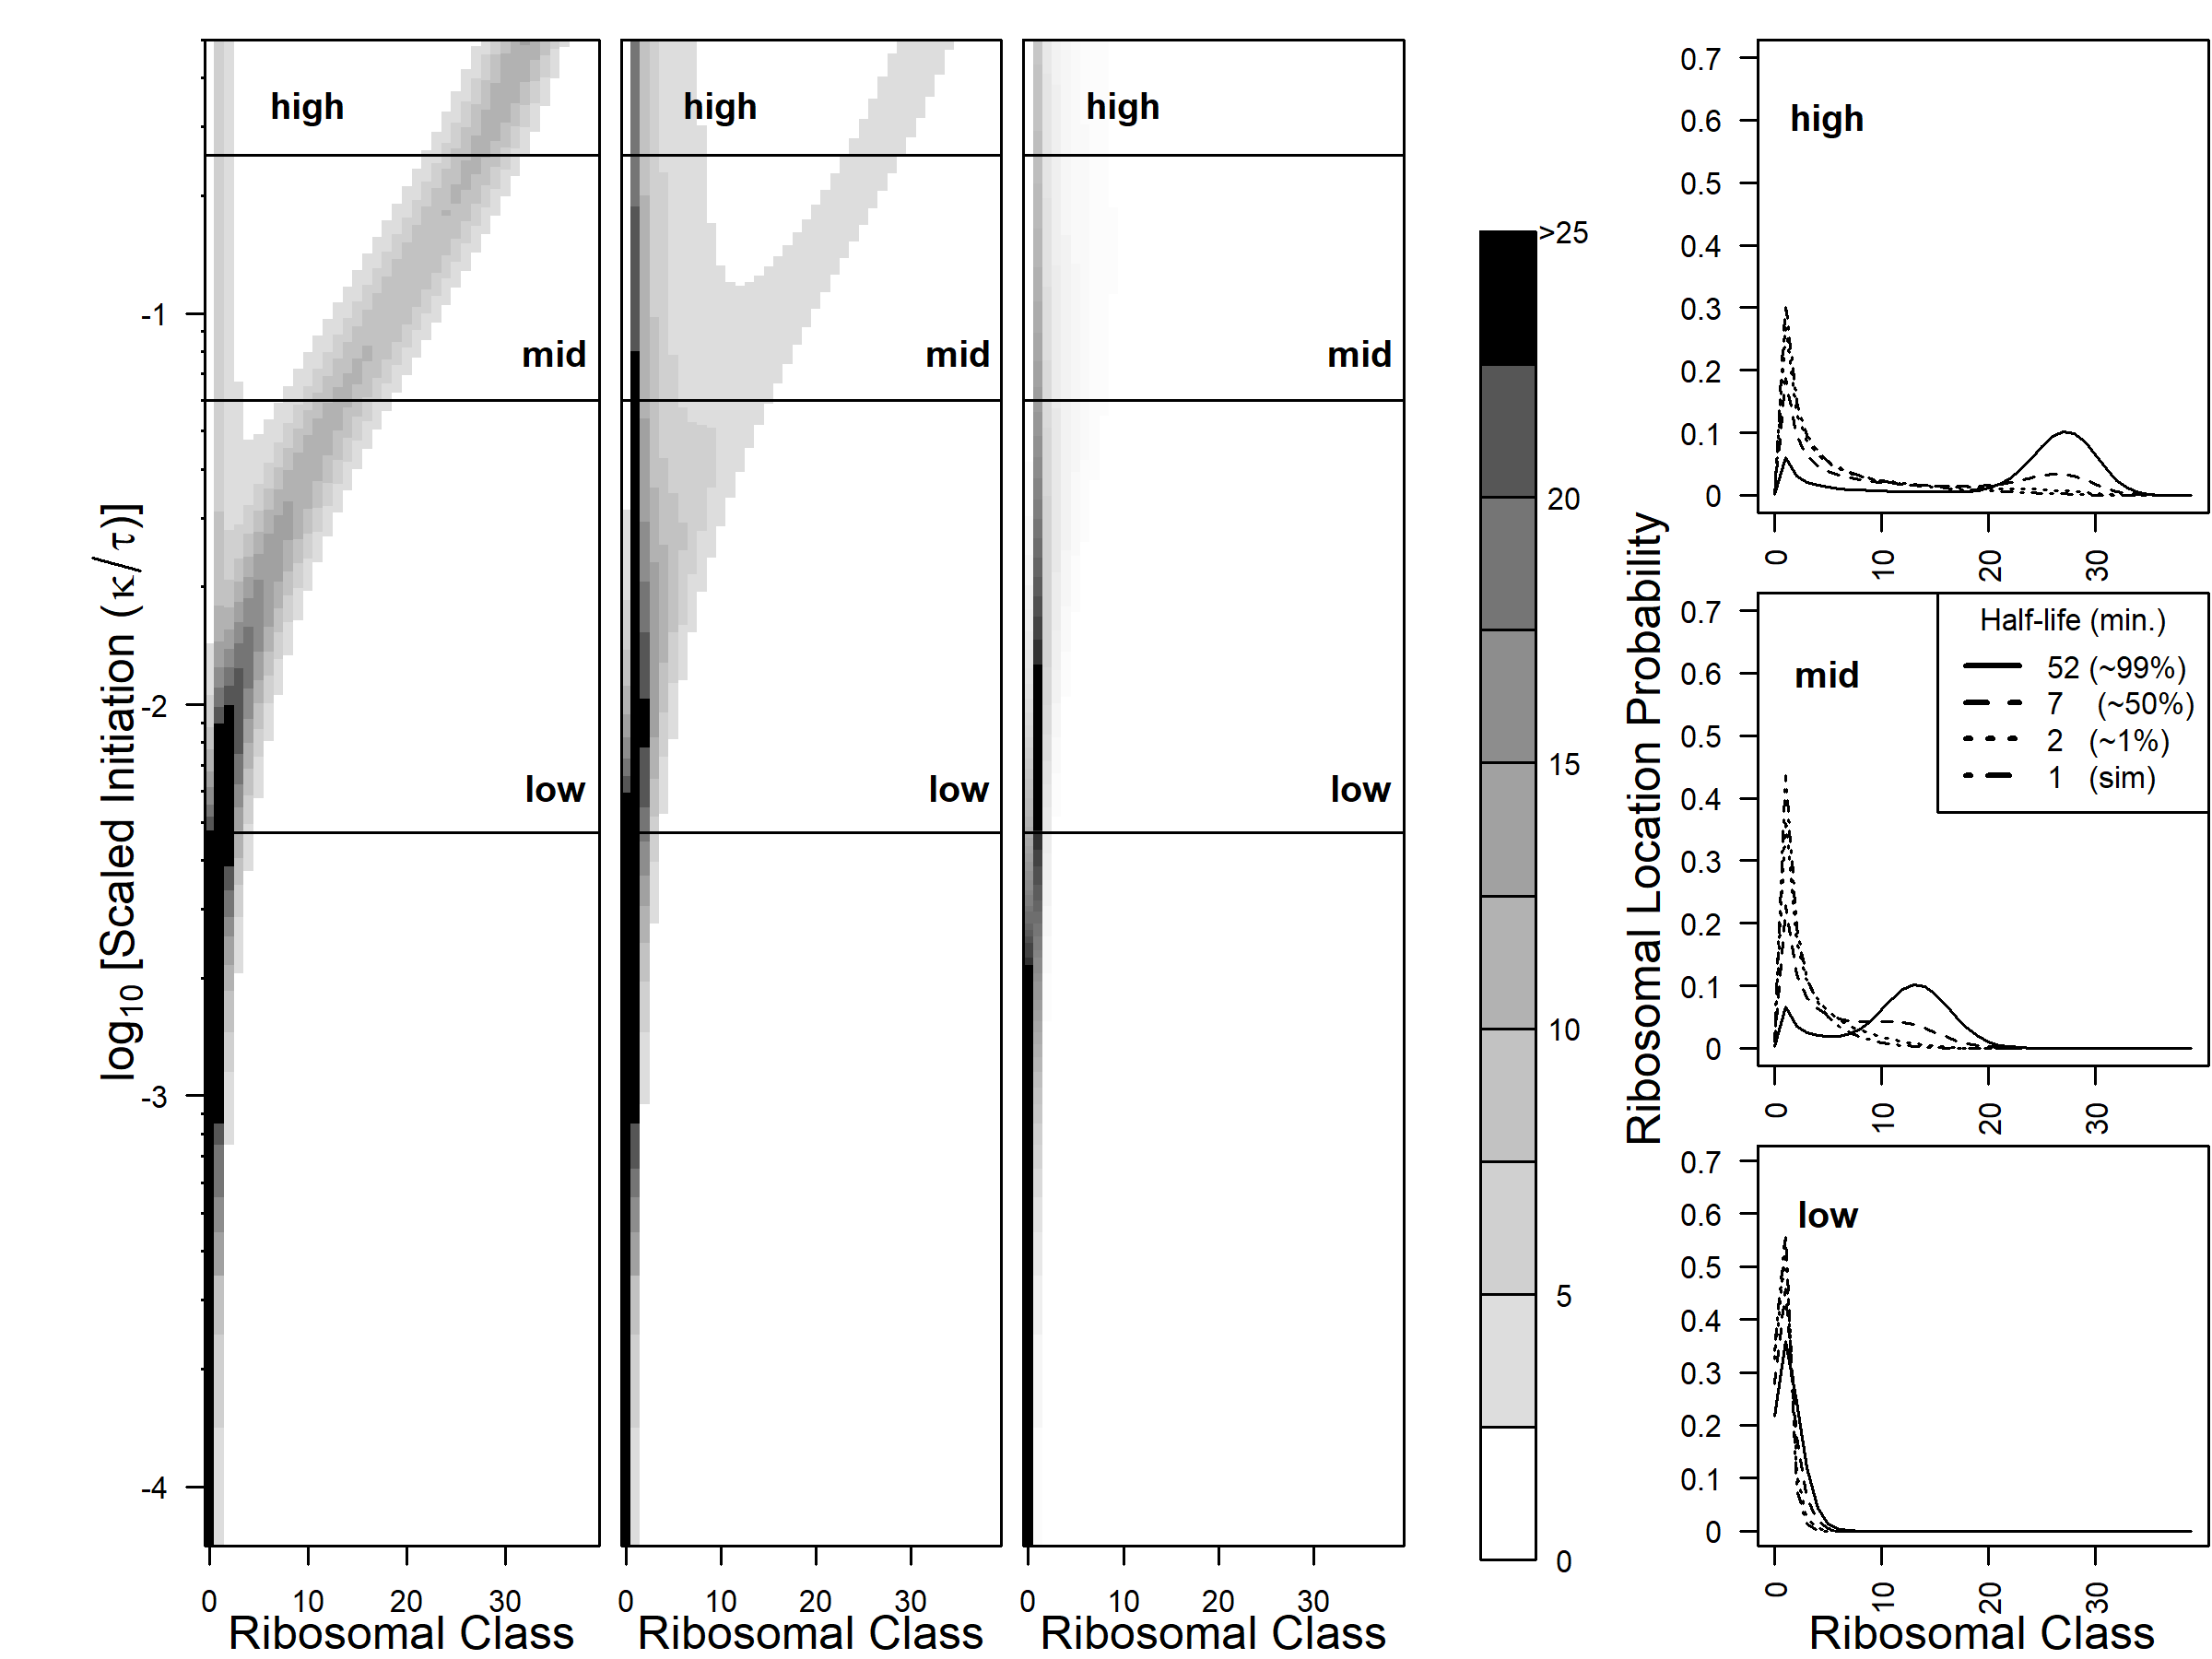
\includegraphics[width=150mm]{Images/2023-06-28_Figure2_Marking_Rate_range_medianlength.png}
\caption{Comparison of density independent initiation (DII) and density dependent initiation (DDI)}
%\centering Red: decapped class, Green: capped class, Blue: Total= capped+decapped classes}
\end{figure}



\begin{figure}[ht]
\centering
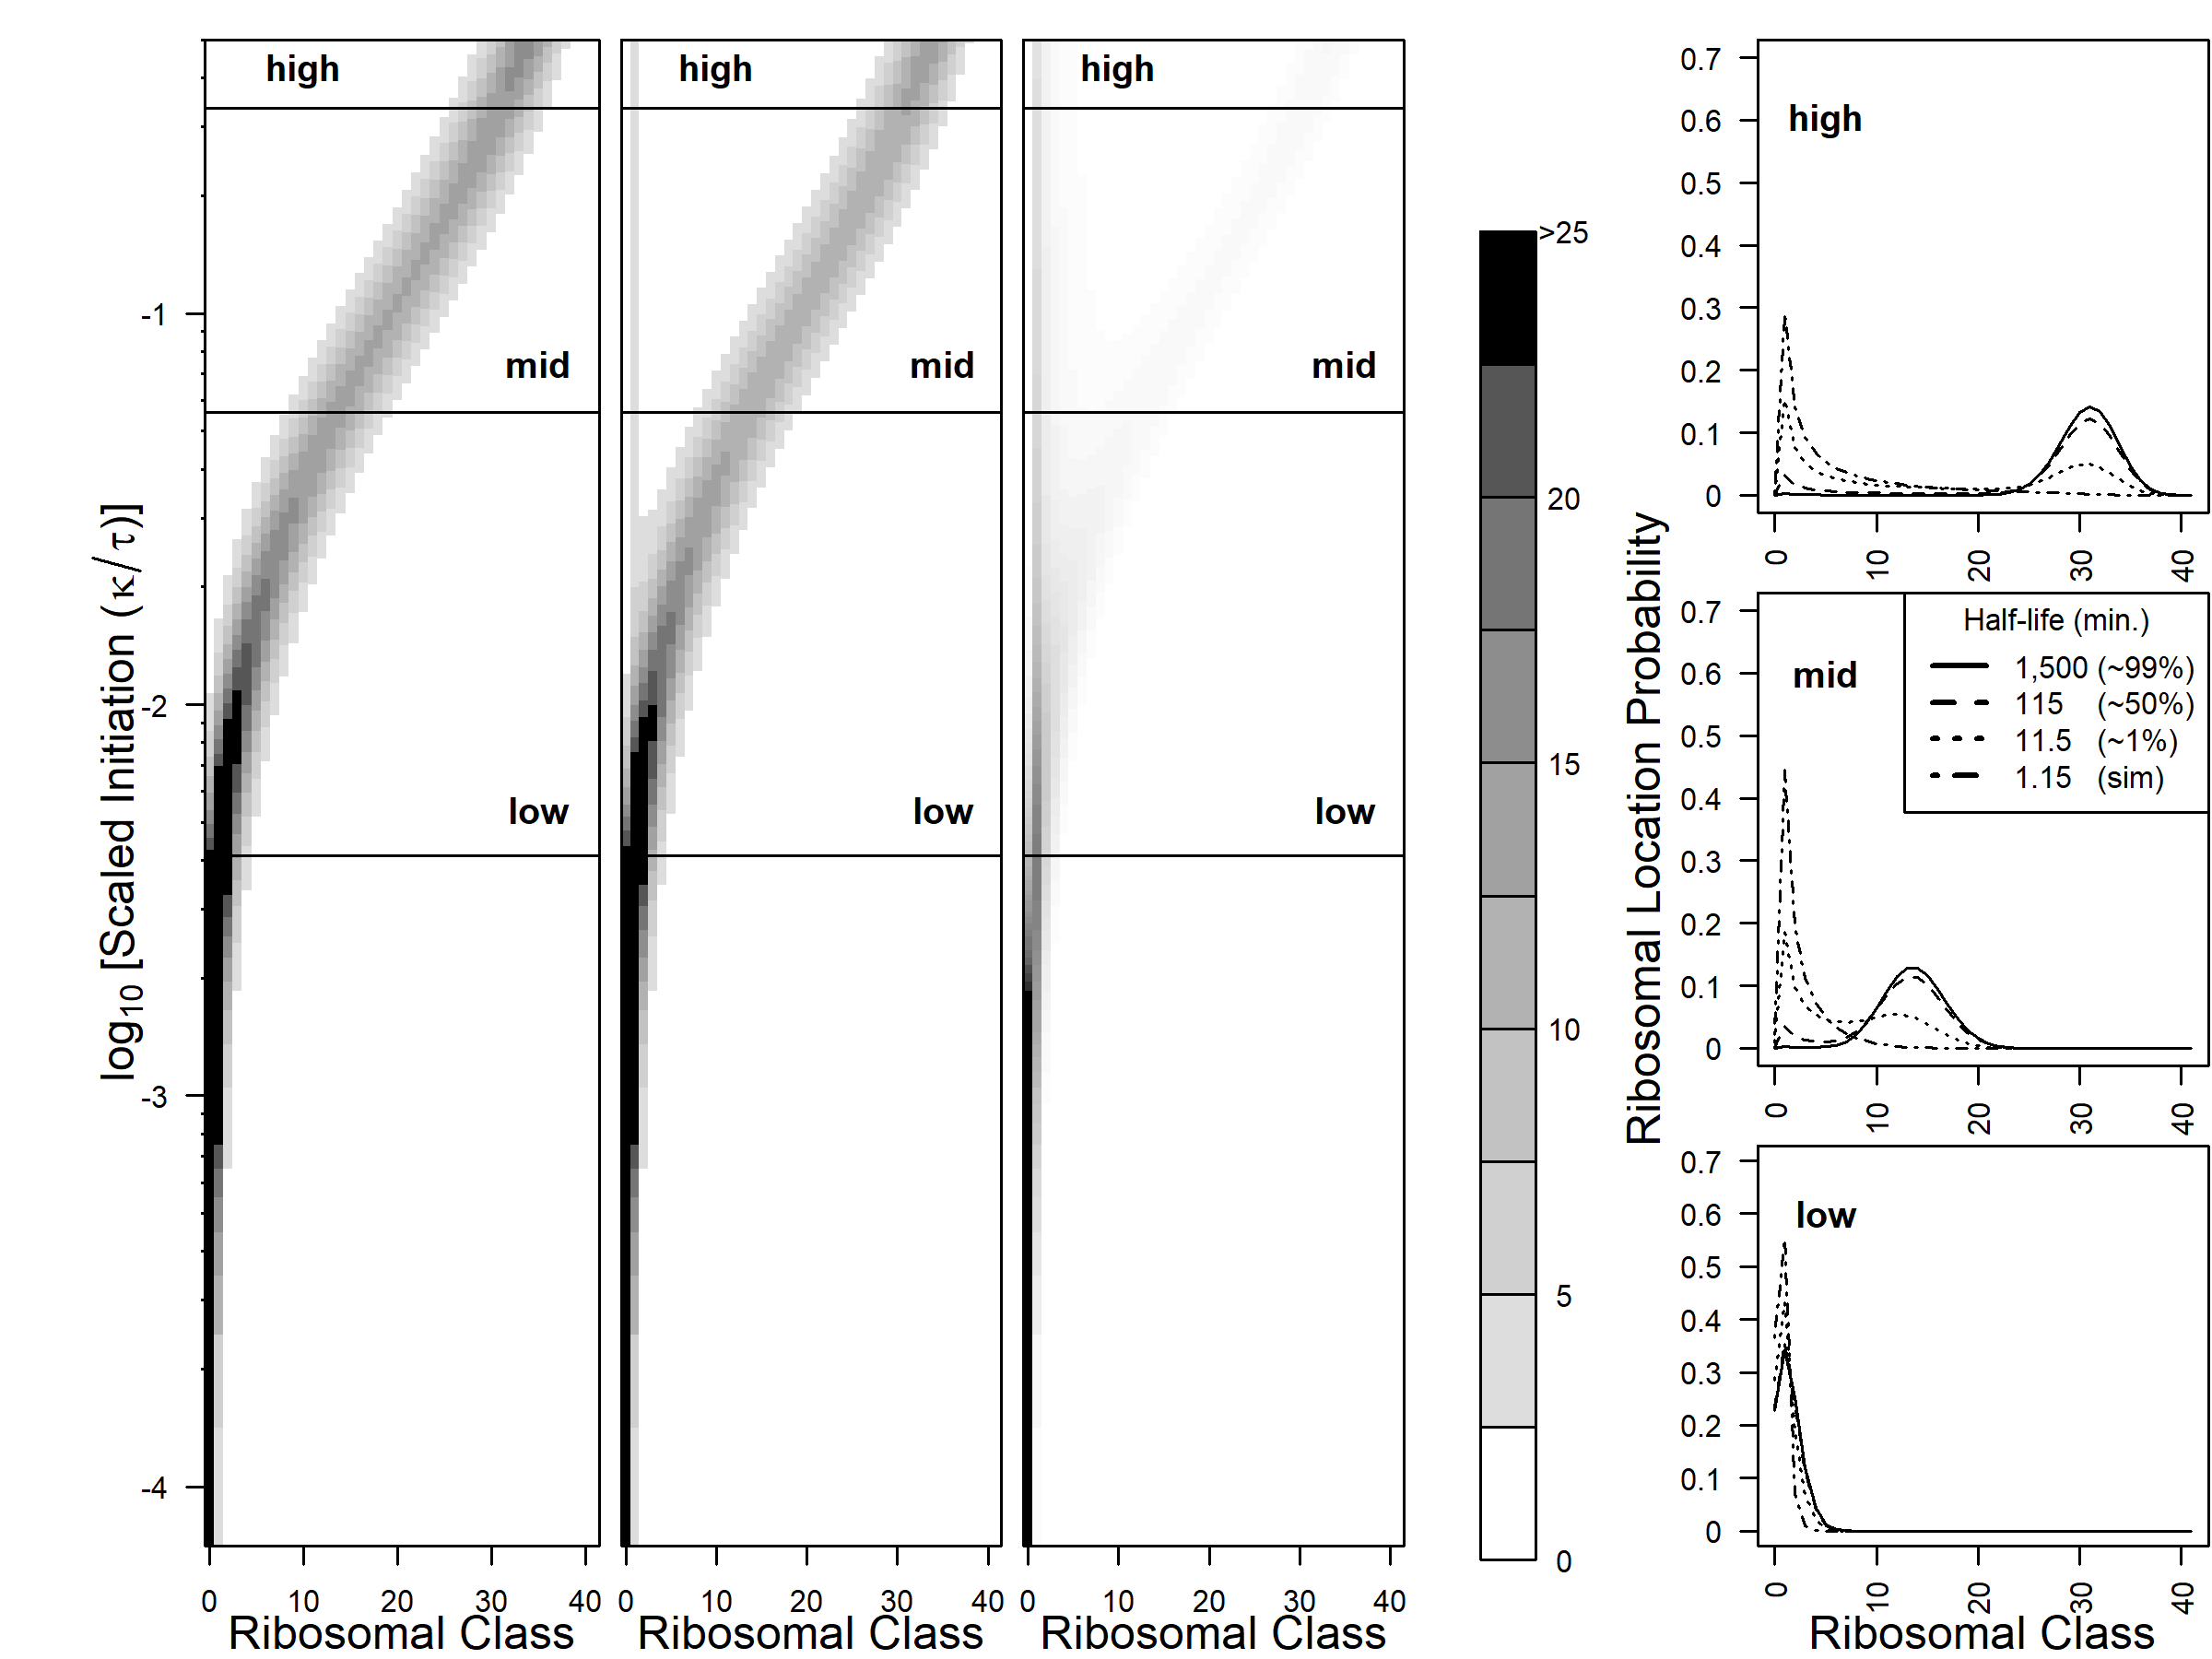
\includegraphics[width=150mm]{Images/2022-10-21_Figure2_Marking_Rate_range_medianlength.png}
\caption{Comparison of density independent initiation (DII) and density dependent initiation (DDI)}
%\centering Red: decapped class, Green: capped class, Blue: Total= capped+decapped classes}
\end{figure}






\begin{figure}[ht]
\centering
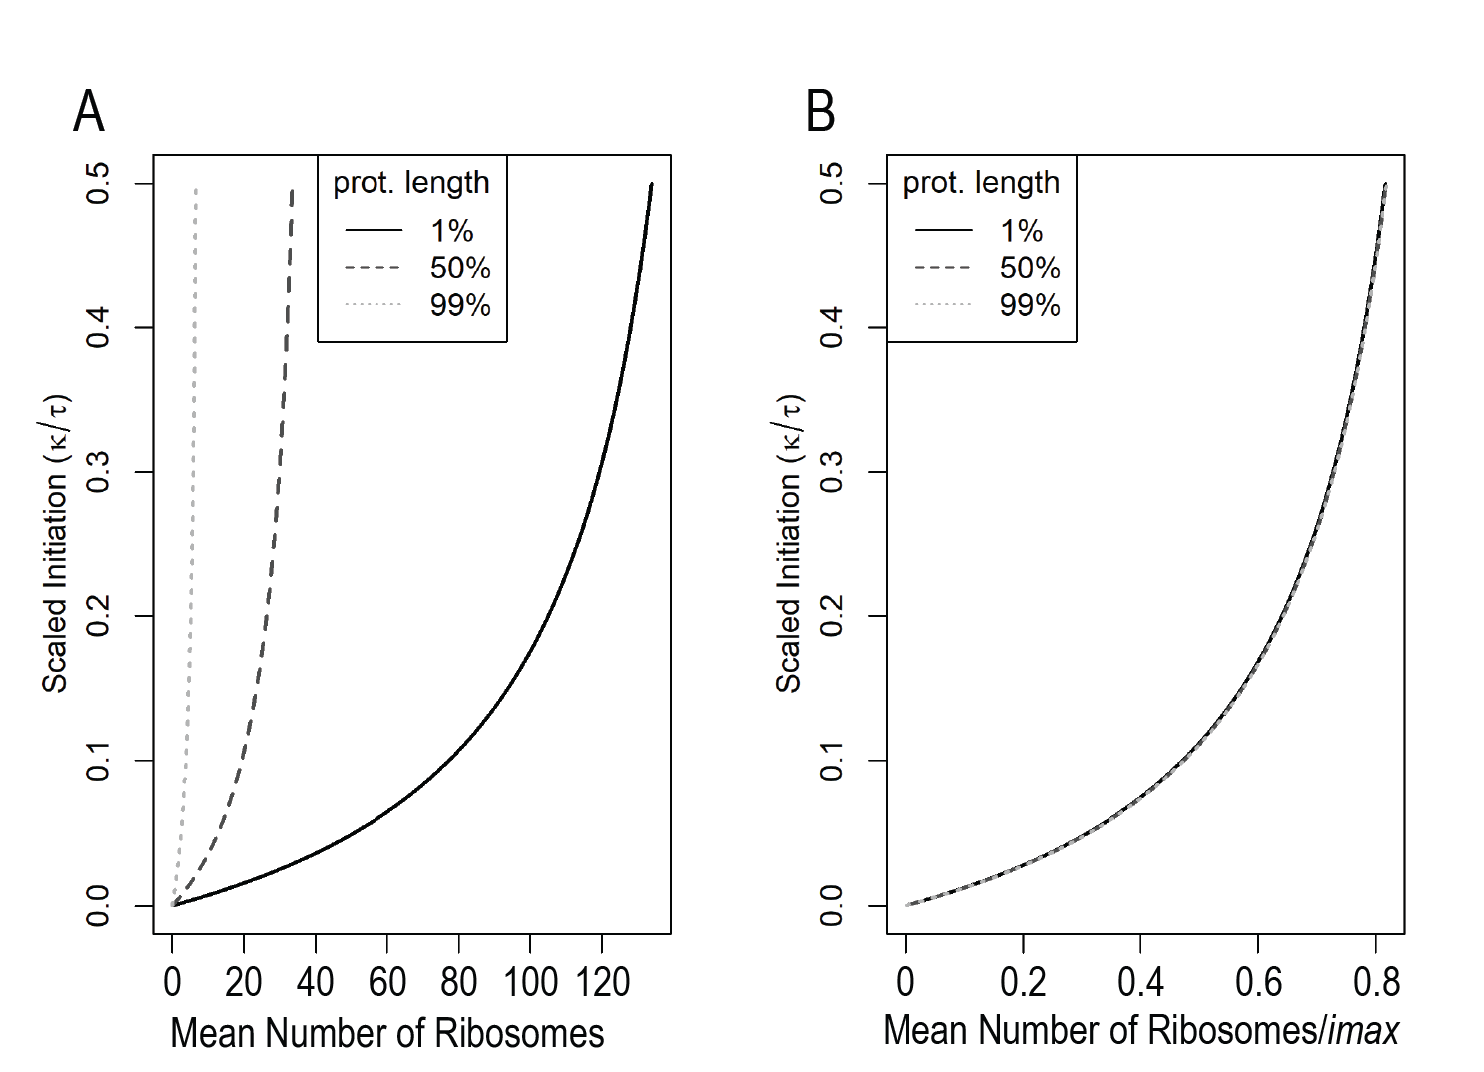
\includegraphics[width=120mm]{Images/2023-07-04_length_independence.png}
\caption{Comparison of density independent initiation (DII) and density dependent initiation (DDI)}
%\centering Red: decapped class, Green: capped class, Blue: Total= capped+decapped classes}
\end{figure}

\begin{figure}[ht]
\centering
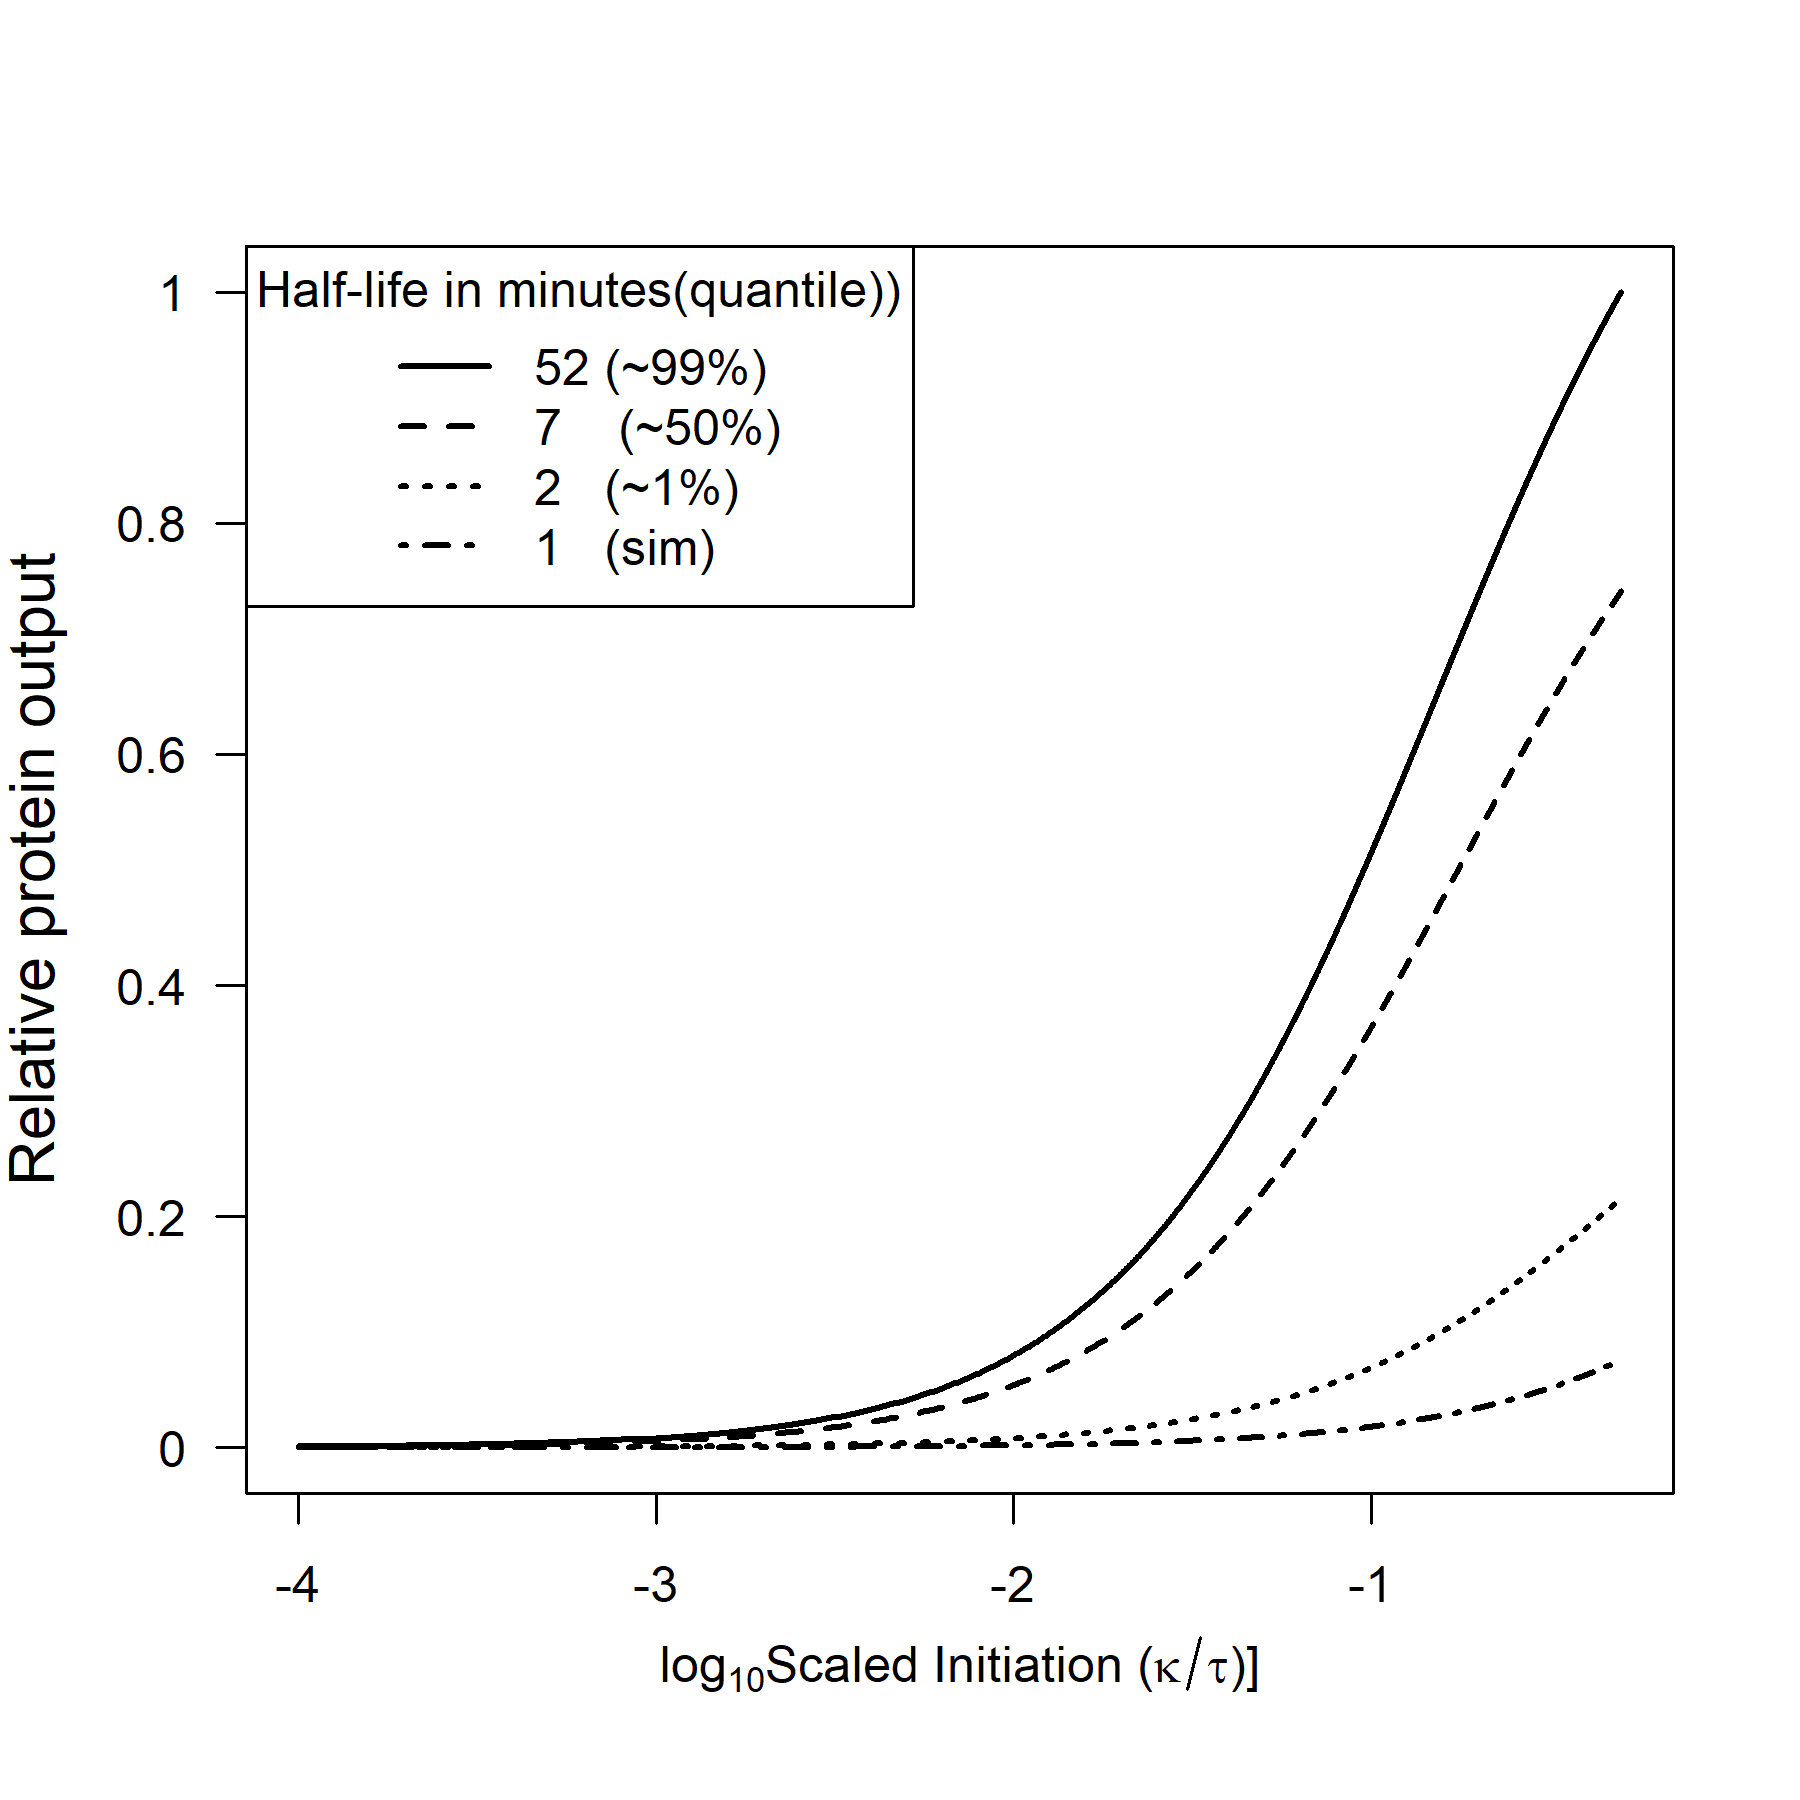
\includegraphics[width = 120mm]{Images/protein_production_stacked_log.png}
\caption{Comparison of density independent initiation (DII) and density dependent initiation (DDI)}
%\centering Red: decapped class, Green: capped class, Blue: Total= capped+decapped classes}
\end{figure}









%most interesting idea I have at the moment is the idea of effective Imax. While our model does not explicitly account for any of the mechanisms or positions of the ribosomes on a transcript, it does predict behavior for hypothetical transcripts. We currently are running on the assumption that one of the determining parameters is the average elongation rate across a transcript. This very well might not be true as 

%Result 1: Longer genes must be translated less efficiently than shorter genes with especially if there is a maximal intitaion/elongation/translation rate. however longer genes might also be more sensitive.  Sensitivity of Translational regulation based on gene size and intiation rate. From results 


%Result 2: Explore the rate limiting effects of tau (geometric,arithmetic sequence dependence) and mu on mean ribosome loading.


%Result 3: decapped class has only a limited effect of the total distribution of mRNAs and overall protein production.


%Result 4: Is translation density dependent or independent? Under which conditions would density start having an effect. 

%Where is translation tuned to? low mid high Translation? Which parameters can have a greater effect. There has to be a maximum speed for all processes (initiation elongation). Test for robustness of protein output vs ranges of these parameters. Does having an early slow stretch of codons effectively shorten a gene's imax?


%Header for result
%First sentence of paragraph
%last sentence of paragraph

%4-5 key  findings due on Monday
%outline due on Wednesday

%Definitions of load vs density vs efficiency vs production rate











%Tau prime is the rate at which ribosomes leave the transcript.
%For a transcript with one ribosome tau prime is the sum of all the individual steps it took the ribosome to get to the stop codon. Since we are not modeling the actual elongation process step by step (and thus mechanistically ignoring pausing or ribosome collisions) we can easily calculate this rate by multiplying the number of codons in gene i by the average translation elongation speed for gene i. 
%For example in a 900 nucleotide long gene will produce a 300 amino acid long protein. If the average elongation rate of the protein is 3 aa/sec, the translation of one protein will take 300aa/3aa/s = 100 s.
%100 seconds is the residence time of a ribosomes on transcript j of gene i. If there are 2 ribosomes the residency time will halve and be 50s. 3 ribosomes = 33.33s, 4 25s and so on. 
%To get the rate of ribosomes leaving the transcript then we will take the reciprocal of this. The leaving rate for 1 ribosome is 1/100 or 0.01. For 2 it is 0.02, for 3, 0.03, and4 0.04 and so on. If every codon was populated by a ribosome (which is physically impossible since a ribosome occupies roughly 9 codons), then the leaving rate would equal the average elongation rate. However, the maximal leaving rate is now imax*termination rate of 1 ribosome. i.e. (imax/#codons)*tau. Or  1/9 tau
%The equation for the residence time is:
%τ'=codons/i*τfor i=1,2,…,imax
%The equation for the termination rate is:
%\tau^\ast=1/\tau^'=i\ast\tau/\left(#codons\right);\ for\ i=0,1,2,\ldots,i_{max}
%Where plain tau is the average elongation rate for transcript j.






%add new decapped class results here. decapped class in its current formulation is very unpopulated. 


	
%work with an protein with a short medium and long lifespan, low medium and high intitiation rates, low medium high elongation rates and short, medium long length.

%What are some of the important interesting questions.
%What does the parameter space look like?
%	What are the currently known ranges for the parameters of interest and what ribosome densities do they produce.
%		Mu will follow the distribution of half lives found in an organims of  
%	Create parameter range which is bounded within relistic parameter values. What are the resulting ribosome loads?
%	For more extreme cases what would the parameters have to be? 
%	How does Imax affect the loading?
%	How does kappa interference affect loading?
%
%Half lives. What does each individual process contribute to the half life of transcripts? 
%	capped 
%	decapped 
%		M0* is delta driven
%		All other M* have a set behaivior dependent on the distribution of transcripts in capped.
%What processes does our current model mimic? What does it miss out? 


 








% without interference if kappa is small relative to tau then interference doesn't matter. if kappa is large what is the distribution? How does increasing mu affect it.

%
%\newpage
%
%\part{Interpreting Data and Mapping the Model to Experimental Data}
%
%
%%\section{Determination of Solutions at Steady-State in Both the Continuous
%%and Discrete Models}
%
%%({*}{*} This should include some of the writing above, including the
%%techniques discussed that utilized the tridiagonal form of the matrix
%%and also using the determinant-adjoint technique for inverting the
%%matrix. {*}{*})
%
%
%\section{Interpreting Experimental Data}
%
%This section will discuss the technique used to interpret the experimental
%data for the distribution of polysomes.  The data being considered here is the work of \emph{J. Guan,} and \emph{A. VonArnim , University of Tennesse - Knoxville}.
%
%
%\subsection{Absorbance Data}
%
%Absorbance data has been generated by a variety of researchers to
%quantify the abundance of different classes of polysomes. This data is often broken down into polysomal
%fractions. The number of fractions can vary depending on the researcher;
%10 to 12 fractions is fairly common in the literature. It is also
%customary to lump the first fractions together into a single non-polysomal
%class. This class includes bare mRNA, those that have ribosomes still
%in the process of binding completely for translation, and those that
%have a single ribosome bound. This non-polysomal class can have up
%to four fractions included in it. A similiar phenonmenon takes place
%in the final fractions. Theoretically, the maximum number of ribosomes
%that can be bound is related to the length of the mRNA. This means
%there can be upwards of forty different mRNA classes (this number
%is related to \imax in the discrete model and $n$ in the continuous
%model). So with 12 fractions and 40 mRNA classes, there is necessarily
%an overlap of classes in each fraction.
%
%The absorbance data itself is reported as a the $log_{2}$ of integral
%of absorbance in each fraction.
%
%
%\subsection{Data Interpretation Techniques}
%
%In interpreting the data there are multiple elements that need to
%be considered first before the abundances estimated by the model can
%be matched up with the UV profiles. A function to relate mRNA class
%to the mean distance travelled in the profile is one piece of information
%that is needed. Also, an estimate of the variance in this travel distance
%is also needed. If a function is to be written to estimate these values,
%one must also know the total length of the UV-Profile, and the background,
%or baseline, amount of fluoresence.
%
%
%\subsubsection{Assumption of Normality and Determiniation of Distribution Parameters}
%
%If we assume that the distribution of mRNA of a given class in the
%UV profile is normally distributed with mean $\mu$and variance $\sigma$,
%then there are graphical techniques that can be used to determine
%these constants directly from UV-Profile diagrams.
%
%Mean distance traveled in the UV Profile is estimated by measuring
%the distance of the peaks in the profile from the ``origin'' in
%the profile (where the origin represents 0\% absorbance and 0 distance
%travelled). This was done by importing the PDF image of the UV-Profile
%into \emph{Mathematica} and then using the standard \emph{'get-coordinates'}
%graphing tool. This work took place under the asssumption that the
%first visible peak in the UV-Profile was from the mRNA class with
%2 ribosomes bound. The coordinates of each distinguishable peak thereafter
%was also found and this data was used to fit a saturating function
%whose maximum value was given by the total length of the UV-Profile.
%The function fitting was performed in \emph{Mathematica }using \emph{'FindFit'}.
%
%The variance was determined by gathering points from the different
%peaks and utilizing the property of the Normal distribution that the
%2nd derivative is related to the curvature of the function. A quadratic
%function was fit to each peak and then the second deriative was found
%and equated to the second derivative of the probability distribution
%function of the Normal distribution. In this way, the distribution
%parameter $\sigma$ was able to be found. Then with estimates of $\sigma$from
%each distinguishable peak in the profile, a function was fit in order
%to estimate $\sigma$ as function of the polysomal class.
%
%Using the estimated values for mean and variance, denoted $\mu_{est}(i)$
%and $\sigma_{est}(i)$ respectively, a mixed PDF was created to mimic
%the UV-Profile. The mixed PDF is comprised of the normal distributions
%$N_{i}(\mu_{est}(i),\sigma_{est}(i))$ and is denoted as $M_{pdf}(N_{i}).$
%
%
%\subsubsection{Connecting the Model to Absorbance Data}
%
%With a function created to mimic the UV-Profile image, the next step
%is to use the absorbance Data to estimate parameters in the model.
%The assumption is made that the height of each peak (and necessarily
%the $log_{2}$of the integral in a fraction) in the UV-Profile is
%proportional to the abundance of each polysomal class. The distribution
%of these abundances is what the model predicts, and so within the
%model we see that the fluoresence in a fraction can be viewed as a
%function of the model parameters and the distribution parameters.
%Letting $\Lambda$represent the vector of model parameters, and $Y_{j}$
%represent the measured absorbance data in fraction $j,$we have
%the following relationship:
%\[
%Y_{j}\propto log_{2}(\sum_{i}\int_{j}^{j+1}m_{tot}(i,\Lambda)\, N_{i}(\mu_{est}(i),\sigma_{est}(i))di)
%\]
%
%
%This states that the amount of absorbance in fraction $j$ is proportional
%to the integral of each Normal function on that fraction times the
%abundance calculated from the model, since each normal function is
%not isolated completely to a fraction, we need to sum the contributions
%from all the functions, which is why the summation over all values
%of $i$ is needed in the relationship. This proportionality is lays
%the framework for the minimization and estimation of the model parameters,
%$\Lambda.$
%
%
%\subsection{Minimization for Parameter Estimation}
%
%This section will present the motivation for the minimization technique
%utilized in the research thusfar. Based on the assumption of Normally
%distributed error (or noise) in the measurement, minimization of the
%sums of difference in model predictions and measurement squared is
%used. This method maximizes Log-Likelihood for the parameter estimates.
 %
%
%
%\subsubsection{Minimization Scheme}
%
%Definitions of the functions and variables used will be given below.
%Beginning with the definitions and relationship relating the data
%to the model estimations in a fluorsecence fraction, where $j\in J$:
%\begin{description}
%\item [{$f_{j}$:}] True value of absorbance in $j^{th}$ fraction, without
%noise in measurement. This is related to model estimates. When considering
%model estimates of this, it will be written as $(f_{j}|\Lambda)$
%\item [{$F_{j}$:}] Value of absorbance in $j^{th}$ fraction with noise
%added.
%\item [{$\epsilon$:}] The amount measurement error or noise, the difference
%between $f_{j}$ and $F_{j}$
%\end{description}
%Related by the following, under the assumption that the noise in each
%fraction has the same distribution:
%
%\begin{align*}
%F_{j} &= f_{j}\cdot\hat{\epsilon}\\
%log_{2}(F_{j}) &= log_{2}(f_{j})+log_{2}(\hat{\epsilon})\\
%Where & \, & \hat{\epsilon}\sim N(0,\sigma_{\epsilon})
%\end{align*}
%The data being considered is given in $log_{2}$of the absorbance
%in a fraction, so for convenience the following will be used:
%\begin{description}
%\item $G_{j}=Log_{2}(F_{j})$
%\item $g_{j}=Log_{2}(f_{j})$
%\item $\epsilon=Log_{2}(\hat{e})\sim LogNormal(0,\sigma_{\epsilon})$
%\end{description}
%Then, the likelihood of $G_{j}$, is given by the following:
%\begin{align*}
%Lik(G_{j}) &= \dfrac{1}{\sqrt{2\pi\sigma_{\epsilon}}}Exp(-\dfrac{(G_{j}-(g_{j}|\Lambda))^{2}}{2\sigma_{\epsilon}^{2}})
%\end{align*}
%
%
%and the $negative\; loglikelihood$ is given by:
%\begin{equation*}
%-LLik(G_{j})=-\ln(\dfrac{1}{\sqrt{2\pi}})+\ln(\sigma_{\epsilon})+\dfrac{(G_{j}-(g_{j}|\Lambda))^{2}}{2\sigma_{\epsilon}^{2}}
%\end{equation*}
%
%
%The objective function to minimize is then:
%\begin{equation*}
%\min_{j}\; n\ln(\sigma_{\epsilon})+\sum_{j\in J}\dfrac{(G_{j}-(g_{i}|\Lambda))^{2}}{2\sigma_{\epsilon}^{2}}
%\end{equation*}
%
%\section{Results}
%
%This section will include our results from simulation as they become available.
%\part*{Appendix}
%\section*{A1: Example solutions to capped system for ODE formulation at equilibrium}
%\begin{description}
%\item This set of solutions is generated from solving the system of capped ODE at equilibrium directly using \emph{Solve[]} in \emph{Mathematica}
%\item For $\imax=1$
%\item \hspace{5pt} $\left\{M(0)\to \frac{\lambda  (\mu +\tau )}{\mu  (\kappa +\mu +\tau )},M(1)\to \frac{\kappa  \lambda }{\mu  (\kappa +\mu +\tau )}\right\}$
%\item For $\imax=2$ 
%\item \hspace{5pt} $\left\{M(0)\to \frac{\lambda  (\kappa  \mu +(\mu +\tau ) (\mu +2 \tau ))}{\mu  \left(\kappa ^2+2 \kappa  (\mu +\tau )+(\mu +\tau ) (\mu +2 \tau )\right)},M(1)\to \frac{\kappa  \lambda  (\mu +2 \tau )}{\mu  \left(\kappa ^2+2 \kappa  (\mu +\tau )+(\mu +\tau ) (\mu +2 \tau )\right)},M(2)\to \frac{\kappa ^2 \lambda }{\mu  \left(\kappa ^2+2 \kappa  (\mu +\tau )+(\mu +\tau ) (\mu +2 \tau )\right)}\right\}$ 
%\item For $\imax=3$
%\item \hspace{5pt} $\Big\{ M(0)\to \frac{\lambda  \left(\kappa ^2 \mu +2 \kappa  \mu  (\mu +2 \tau )+(\mu +\tau ) (\mu +2 \tau ) (\mu +3 \tau )\right)}{\mu  \left(\tau ^2 (6 \kappa +11 \mu )+3 \tau  (\kappa +2 \mu ) (\kappa +\mu )+(\kappa +\mu )^3+6 \tau ^3\right)},M(1)\to \frac{\kappa  \lambda  (\kappa  \mu +(\mu +2 \tau ) (\mu +3 \tau ))}{\mu  \left(\tau ^2 (6 \kappa +11 \mu )+3 \tau  (\kappa +2 \mu ) (\kappa +\mu )+(\kappa +\mu )^3+6 \tau ^3\right)},$
%\item \hspace{9pt} $ M(2)\to \frac{\kappa ^2 \lambda  (\mu +3 \tau )}{\mu  \left(\tau ^2 (6 \kappa +11 \mu )+3 \tau  (\kappa +2 \mu ) (\kappa +\mu )+(\kappa +\mu )^3+6 \tau ^3\right)},M(3)\to \frac{\kappa ^3 \lambda }{\mu  \left(\tau ^2 (6 \kappa +11 \mu )+3 \tau  (\kappa +2 \mu ) (\kappa +\mu )+(\kappa +\mu )^3+6 \tau ^3\right)} \Big\} $
%\item For $\imax=4$
%\item \hspace{5pt} $\Big\{M(0)\to \frac{\lambda  \left(\mu  \tau ^2 (18 \kappa +35 \mu )+5 \mu  \tau  (\kappa +\mu ) (\kappa +2 \mu )+\mu  (\kappa +\mu )^3+50 \mu  \tau ^3+24 \tau ^4\right)}{\mu  \left(2 \tau ^3 (12 \kappa +25 \mu )+\tau ^2 (2 \kappa +5 \mu ) (6 \kappa +7 \mu )+2 \tau  (2 \kappa +5 \mu ) (\kappa +\mu )^2+(\kappa +\mu )^4+24 \tau ^4\right)},$
%\item \hspace{9pt} $M(1)\to \frac{\kappa  \lambda  \left(\kappa ^2 \mu +2 \kappa  \mu  (\mu +3 \tau )+(\mu +2 \tau ) (\mu +3 \tau ) (\mu +4 \tau )\right)}{\mu  \left(2 \tau ^3 (12 \kappa +25 \mu )+\tau ^2 (2 \kappa +5 \mu ) (6 \kappa +7 \mu )+2 \tau  (2 \kappa +5 \mu ) (\kappa +\mu )^2+(\kappa +\mu )^4+24 \tau ^4\right)},$
%\item \hspace{9pt} $M(2)\to \frac{\kappa ^2 \lambda  (\kappa  \mu +(\mu +3 \tau ) (\mu +4 \tau ))}{\mu  \left(2 \tau ^3 (12 \kappa +25 \mu )+\tau ^2 (2 \kappa +5 \mu ) (6 \kappa +7 \mu )+2 \tau  (2 \kappa +5 \mu ) (\kappa +\mu )^2+(\kappa +\mu )^4+24 \tau ^4\right)},$\item \hspace{9pt} $M(3)\to \frac{\kappa ^3 \lambda  (\mu +4 \tau )}{\mu  \left(2 \tau ^3 (12 \kappa +25 \mu )+\tau ^2 (2 \kappa +5 \mu ) (6 \kappa +7 \mu )+2 \tau  (2 \kappa +5 \mu ) (\kappa +\mu )^2+(\kappa +\mu )^4+24 \tau ^4\right)},$
%\item \hspace{9pt} $M(4)\to \frac{\kappa ^4 \lambda }{\mu  \left(2 \tau ^3 (12 \kappa +25 \mu )+\tau ^2 (2 \kappa +5 \mu ) (6 \kappa +7 \mu )+2 \tau  (2 \kappa +5 \mu ) (\kappa +\mu )^2+(\kappa +\mu )^4+24 \tau ^4\right)}\Big\}$
%
%\item Recall that the decapped solutions are solved completely in terms of the capped solutions using equation (7).
%
%\end{description}

\end{document}
